%%%%%%%%%%%%%%%%%%%%%%%%%%%%%%%%%%%%%%%%%
% Beamer Presentation
% LaTeX Template
% Version 1.0 (10/11/12)
%
% This template has been downloaded from:
% http://www.LaTeXTemplates.com
%
% License:
% CC BY-NC-SA 3.0 (http://creativecommons.org/licenses/by-nc-sa/3.0/)
%
%%%%%%%%%%%%%%%%%%%%%%%%%%%%%%%%%%%%%%%%%

%----------------------------------------------------------------------------------------
%	PACKAGES AND THEMES
%----------------------------------------------------------------------------------------

\documentclass{beamer}

\mode<presentation> {

% The Beamer class comes with a number of default slide themes
% which change the colors and layouts of slides. Below this is a list
% of all the themes, uncomment each in turn to see what they look like.

%\usetheme{default}
%\usetheme{AnnArbor}
%\usetheme{Antibes}
%\usetheme{Bergen}
%\usetheme{Berkeley}
%\usetheme{Berlin}
%\usetheme{Boadilla}
%\usetheme{CambridgeUS}
%\usetheme{Copenhagen}
%\usetheme{Darmstadt}
%\usetheme{Dresden}
%\usetheme{Frankfurt}
%\usetheme{Goettingen}
%\usetheme{Hannover}
%\usetheme{Ilmenau}
%\usetheme{JuanLesPins}
%\usetheme{Luebeck}
\usetheme{Madrid}
%\usetheme{Malmoe}
%\usetheme{Marburg}
%\usetheme{Montpellier}
%\usetheme{PaloAlto}
%\usetheme{Pittsburgh}
%\usetheme{Rochester}
%\usetheme{Singapore}
%\usetheme{Szeged}
%\usetheme{Warsaw}

% As well as themes, the Beamer class has a number of color themes
% for any slide theme. Uncomment each of these in turn to see how it
% changes the colors of your current slide theme.

%\usecolortheme{albatross}
%\usecolortheme{beaver}
%\usecolortheme{beetle}
%\usecolortheme{crane}
%\usecolortheme{dolphin}
%\usecolortheme{dove}
%\usecolortheme{fly}
%\usecolortheme{lily}
%\usecolortheme{orchid}
%\usecolortheme{rose}
%\usecolortheme{seagull}
%\usecolortheme{seahorse}
%\usecolortheme{whale}
%\usecolortheme{wolverine}

%\setbeamertemplate{footline} % To remove the footer line in all slides uncomment this line
%\setbeamertemplate{footline}[page number] % To replace the footer line in all slides with a simple slide count uncomment this line

%\setbeamertemplate{navigation symbols}{} % To remove the navigation symbols from the bottom of all slides uncomment this line
}

\usepackage{graphicx} % Allows including images
\usepackage{booktabs} % Allows the use of \toprule, \midrule and \bottomrule in tables
\usepackage{xcolor}
\usepackage{tikz}
\usepackage[tikz]{bclogo}
\usepackage[absolute,overlay]{textpos}
\usepackage{tcolorbox}
\usepackage{makecell}
\usepackage{multirow}

\newcommand{\imp}[1]{{\color{red}{#1}}}
\newcommand{\remark}[1]{{\color{blue}{#1}}}
\newcommand{\atten}[1]{{\color{green}{#1}}}
\newcommand\Fontvi{\fontsize{9}{10.2}\selectfont}

\newcommand{\tfidf}{\emph{tf-idf}}
\newcommand{\NMF}{\emph{NMF}}

\definecolor{mygreen}{rgb}{0, 0.5, 0}
\newcommand{\PA}[1]{{\color{mygreen}{#1}}}


%----------------------------------------------------------------------------------------
%	TITLE PAGE
%----------------------------------------------------------------------------------------

\title[Short title]{More State of the Art} % The short title appears at the bottom of every slide, the full title is only on the title page

\author{Pegah ALIZADEH} % Your name
\institute[GREYC] % Your institution as it will appear on the bottom of every slide, may be shorthand to save space
{
University of Caen Normandy (Labratoire GREYC) \\ % Your institution for the title page
\medskip
\textit{pegah.alizadeh@unicaen.fr} % Your email address
}
\date{\today} % Date, can be changed to a custom date

\begin{document}

\begin{frame}
\titlepage % Print the title page as the first slide
\end{frame}

\begin{frame}{Outline}
\tableofcontents
\end{frame}

%----------------------------------------------------------------------------------------
%	PRESENTATION SLIDES
%----------------------------------------------------------------------------------------

%------------------------------------------------
\section{Elicitation and Planning in MDPs with Unknown Rewards}
%------------------------------------------------

\begin{frame}
\begin{center}
\textbf{Elicitation and Planning in MDPs with Unknown Rewards}
\end{center}
\end{frame}

%------------------------------------------------
\begin{frame}{Goal and Questions}

\begin{itemize}
\item[-] We are in a \textbf{sequential decision problem}.
\item[-] Users have \textbf{various preferences}.
\item[-] We can \textbf{ask questions} on user's preferences.
\item[-] The optimal policy is computed w.r.t the set of preferences.
\end{itemize}

\begin{bclogo}[arrondi = 0.1, logo=, ombre = true]{}
\begin{itemize}
\item[] {\color{red} GOAL}: Given a sequential decision problem, we wish to find the optimal policy satisfying user priorities by \textbf{asking as few as possible number of queries to users}.
\item[] {\color{red} RESEARCH QUESTIONS}: 

\begin{itemize}
\item\textbf{Reducing the number of queries} to the user 
\item \textbf{Robust policies} for noises answers
\item Applicable method on \textbf{higher MDP sizes}
\item \textbf{Speed up} robust policy computation
\end{itemize}

\end{itemize}
\end{bclogo}

\end{frame}

%------------------------------------------------

\begin{frame}{Markov Decision Processes with Unknown Rewards}
\Fontvi
There are more than one objective in the system. Rewards can not be defined numerically: ~\\
Each objective needs a separate reward: $\forall s,a \;\; r(s, a)=$({\colorbox{green}{\strut comfort} , \colorbox{yellow}{\strut ethic}})
\begin{center}
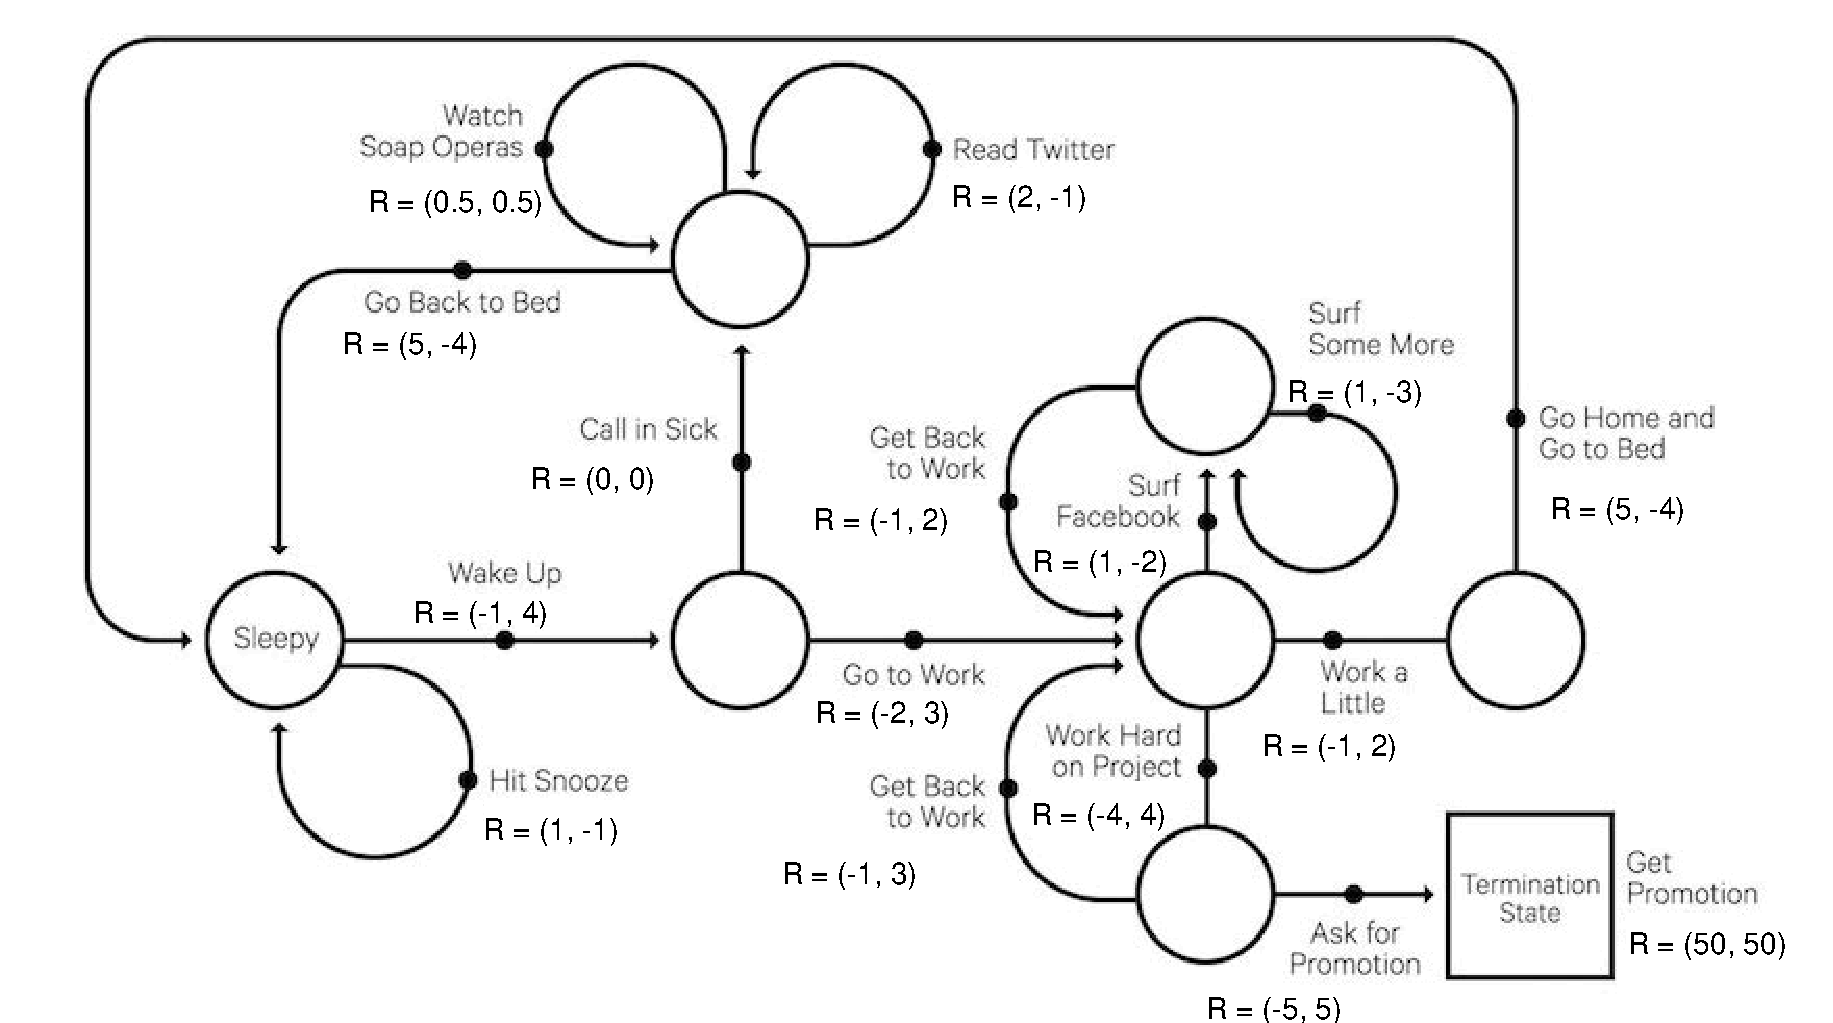
\includegraphics[scale=0.35]{figures-new/mdp-example-cool-2} ~\\
\end{center}

%\pause
%\only<2>{
%\begin{textblock*}{64mm}(32mm,0.25\textheight)
%\begin{tcolorbox}[colback=green!5,colframe=green!40!black]{A Vector-valued MDP (VMDP) is a tuple $<S, A, p, \bar{r}, \gamma, \beta>$ where:}
%
%\begin{itemize}
%\item $S$ set of \atten{states}
%\item $A$ set of \atten{actions}
%\item $P: S \times A \times A \longrightarrow [0,1]$ \alert{transition function}
%\item {\color{red} $\bar r:S \times A \longrightarrow \mathbb{R}^d$ vector reward function}; $d$ is number of objectives or preferences in the model
%\item $\beta: S \longrightarrow [0,1]$ initial states distribution
%\item $\gamma \in [0,1)$ \alert{discount factor}
%\end{itemize}
%
%\end{tcolorbox}
%\end{textblock*}
%}

\end{frame}


%------------------------------------------------

\begin{frame}

A Vector-valued MDP (VVMDP) is a tuple $<S, A, p, \bar{r}, \gamma, \beta>$ where:

\begin{itemize}
\item $S$ set of \remark{states}
\item $A$ set of \remark{actions}
\item $P: S \times A \times A \longrightarrow [0,1]$ \remark{transition function}
\item \remark{$\bar r:S \times A \longrightarrow \mathbb{R}^d$ vector reward function}; $d$ is number of objectives or preferences in the model
\item $\beta: S \longrightarrow [0,1]$ initial states distribution
\item $\gamma \in [0,1)$ \remark{discount factor}
\end{itemize}

\end{frame}

%------------------------------------------------
\begin{frame}{Policies and Vector-valued Functions}

\begin{block}{\alert{Policy}}
A stationary policy $\pi: S \longrightarrow A$ maps each state to an action
\end{block}


\begin{block}{\alert{Vector valued function}} 
Is the expectation of discounted sum of vector rewards $\bar{V}^{\pi} : S \longrightarrow \mathbb{R}^{d}$:
\begin{equation*}
\bar{V}^{\pi} =  \mathbb{E}[\sum_{t=0}^{\infty} \gamma \bar{r}_t \; | \; \pi, \beta ]
\end{equation*}
\end{block}

\begin{block}{}
\alert{Optimal  policy} is the policy with the highest vector-valued function
{\color{mygreen} How to choose the optimal vector among a set of vectors?}
\end{block}

\end{frame}

%%%%%%%%%%%%%%%%%%%%%%%%%%%%%%%%%%%%%%%%%%%%%%%%%%%%%%
\begin{frame}{How the optimal policy is related to the user preferences:}
\Fontvi
\begin{itemize}
\item The preferences of user on objectives are modeled by: {\color{red}$\bar{\lambda}$} 
\item {\color{red}$\bar{\lambda}$} is the user weights over objectives
\item The set of the reward weights {\color{red}$\bar{\lambda}$} can be represented as a polytope: $\Lambda = \{ (\lambda_1, \cdots, \lambda_d) \text{ s.t. } \sum_i \lambda_i = 1\}$
\item The value policy is linear combination of reward weights:
\begin{equation*}
V^{\pi} = \text{ {\color{red}$\bar{\lambda}$}} \cdot \bar{V}^{\pi} % \longrightarrow \pi^* = \text{argmax}_{\pi} \bar{\lambda} \cdot \bar{V}^{\pi}
\end{equation*}
\end{itemize}


\alert{example}: In the driver problem, there are two objectives: {\color{mygreen} Eco-friend} and  {\color{blue} speed-lover}
\begin{itemize}
\item[] {\color{mygreen} Sophie}: prefers a green environment than speed $\bar{\lambda}_{\text{Sophie}} = (0.9, 0.1)$
\item[] {\color{blue} Kevin}: prefers speed that a green environment  $\bar{\lambda}_{\text{Kevin}} = (0.1, 0.9)$
\end{itemize}

\begin{center}
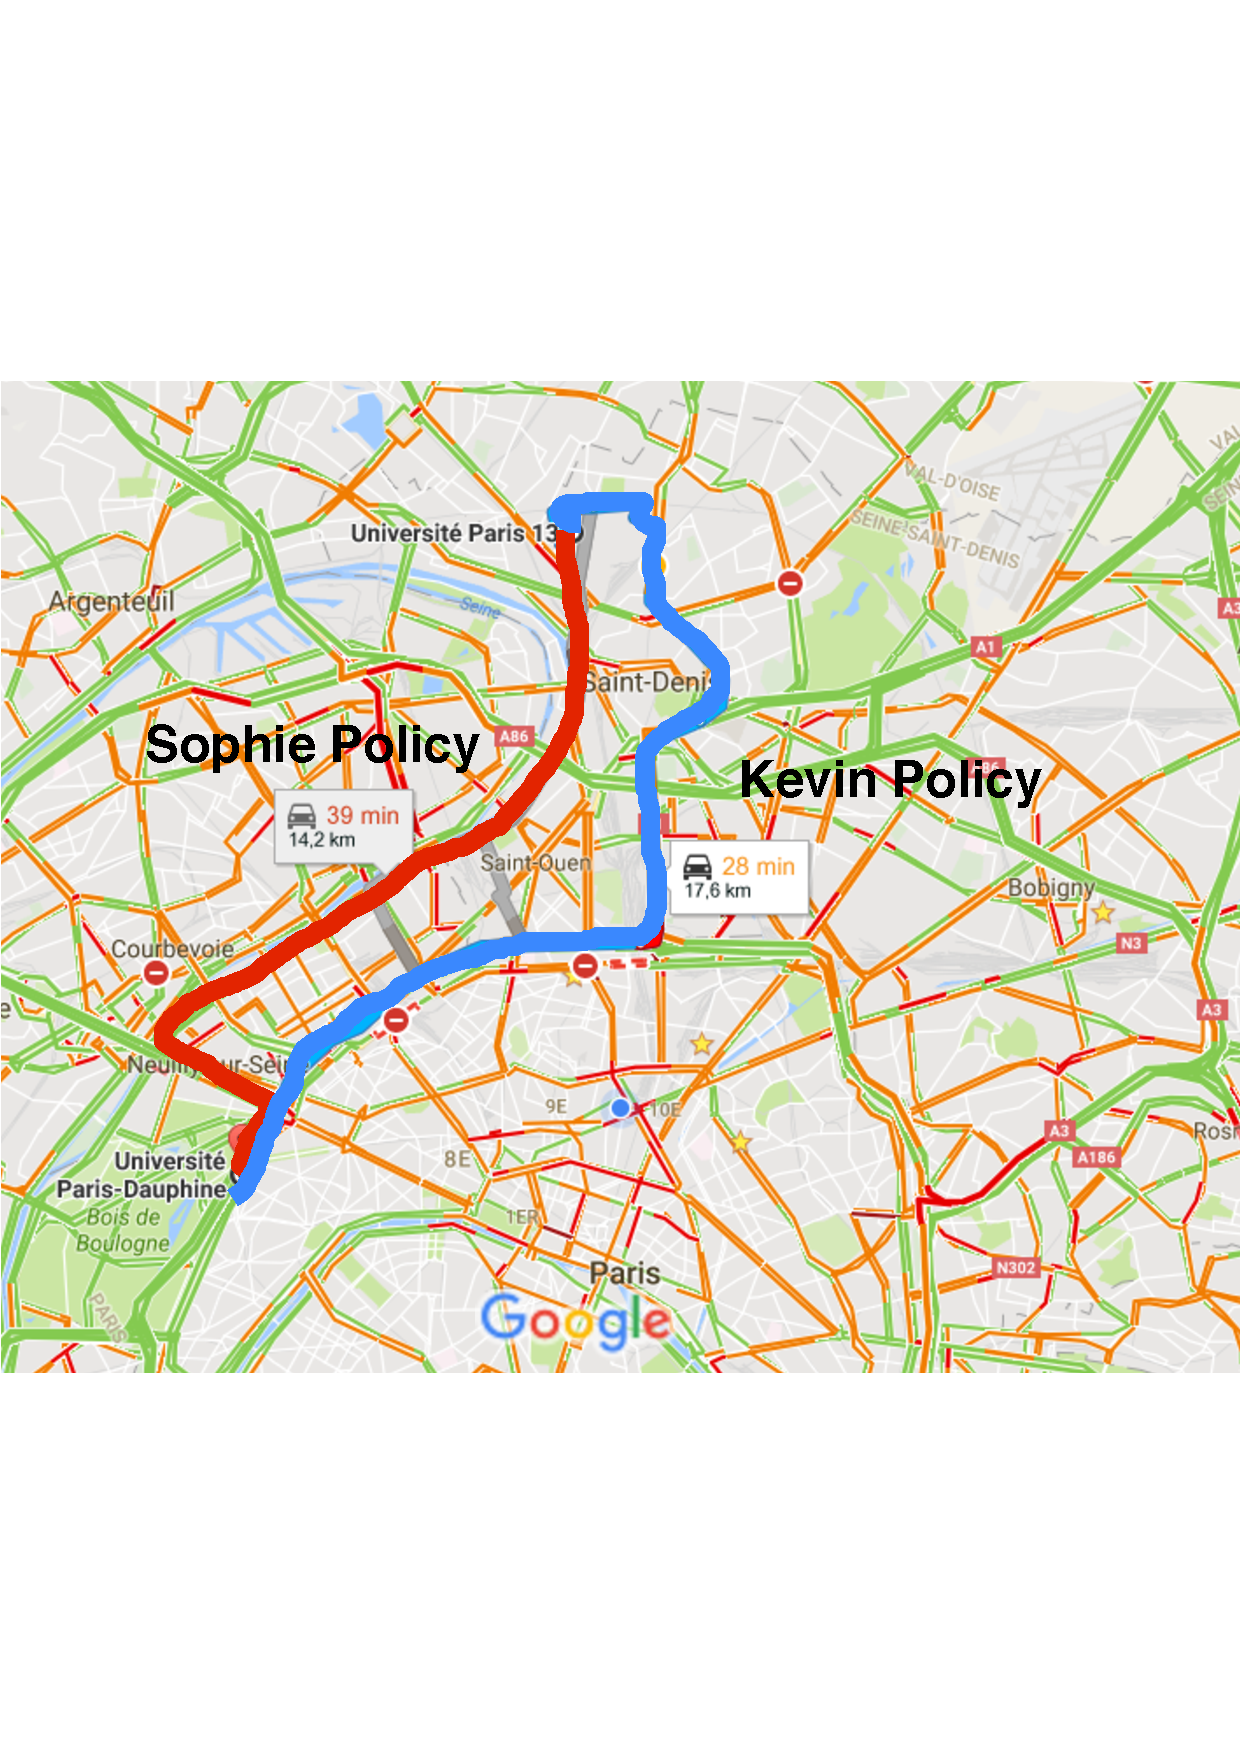
\includegraphics[scale=0.26]{figures-new/user-choise-new}
\end{center}
\end{frame}

%%%%%%%%%%%%%%%%%%%%%%%%%%%%%%%
\begin{frame}
Three main works of my thesis:

\begin{itemize}
 \item \remark{Elicitation}: 
	\begin{itemize}
	\item  Advantage Based Value Iteration algorithm (ABVI)
	 \item Propagation-search method
\end{itemize}	 
 \item \remark{Robust Policy} Selected Random Points Method for accelerating minimax regret computation
\end{itemize}

\end{frame}

%%%%%%%%%%%%%%%%%%%%%%%%%%%%%%%

\begin{frame}
\begin{center}
 \textbf{Elicitation}
\end{center}
\end{frame}

%%%%%%%%%%%%%%%%%%%%%%%%%%%%%%%

\begin{frame}

The designed system based on VMDP:
\begin{itemize}
\item Find the optimal policy by comparing vector-values of policies w.r.t $\Lambda$
\item Reduce $\Lambda$ polytope with querying users.
\end{itemize}
\alert{For instance}, if the user prefers $\underbrace{\text{eco-freind}}_{\lambda_1}$ drive rather that $10 \times \underbrace{\text{speed}}_{\lambda_2}$, one side of $\lambda_1 = 10 \lambda_2$ line in $\Lambda$ polytope is removed. 

\begin{figure}[h!]
\centering
\begin{tikzpicture}
\node[] (img) at (0,0) {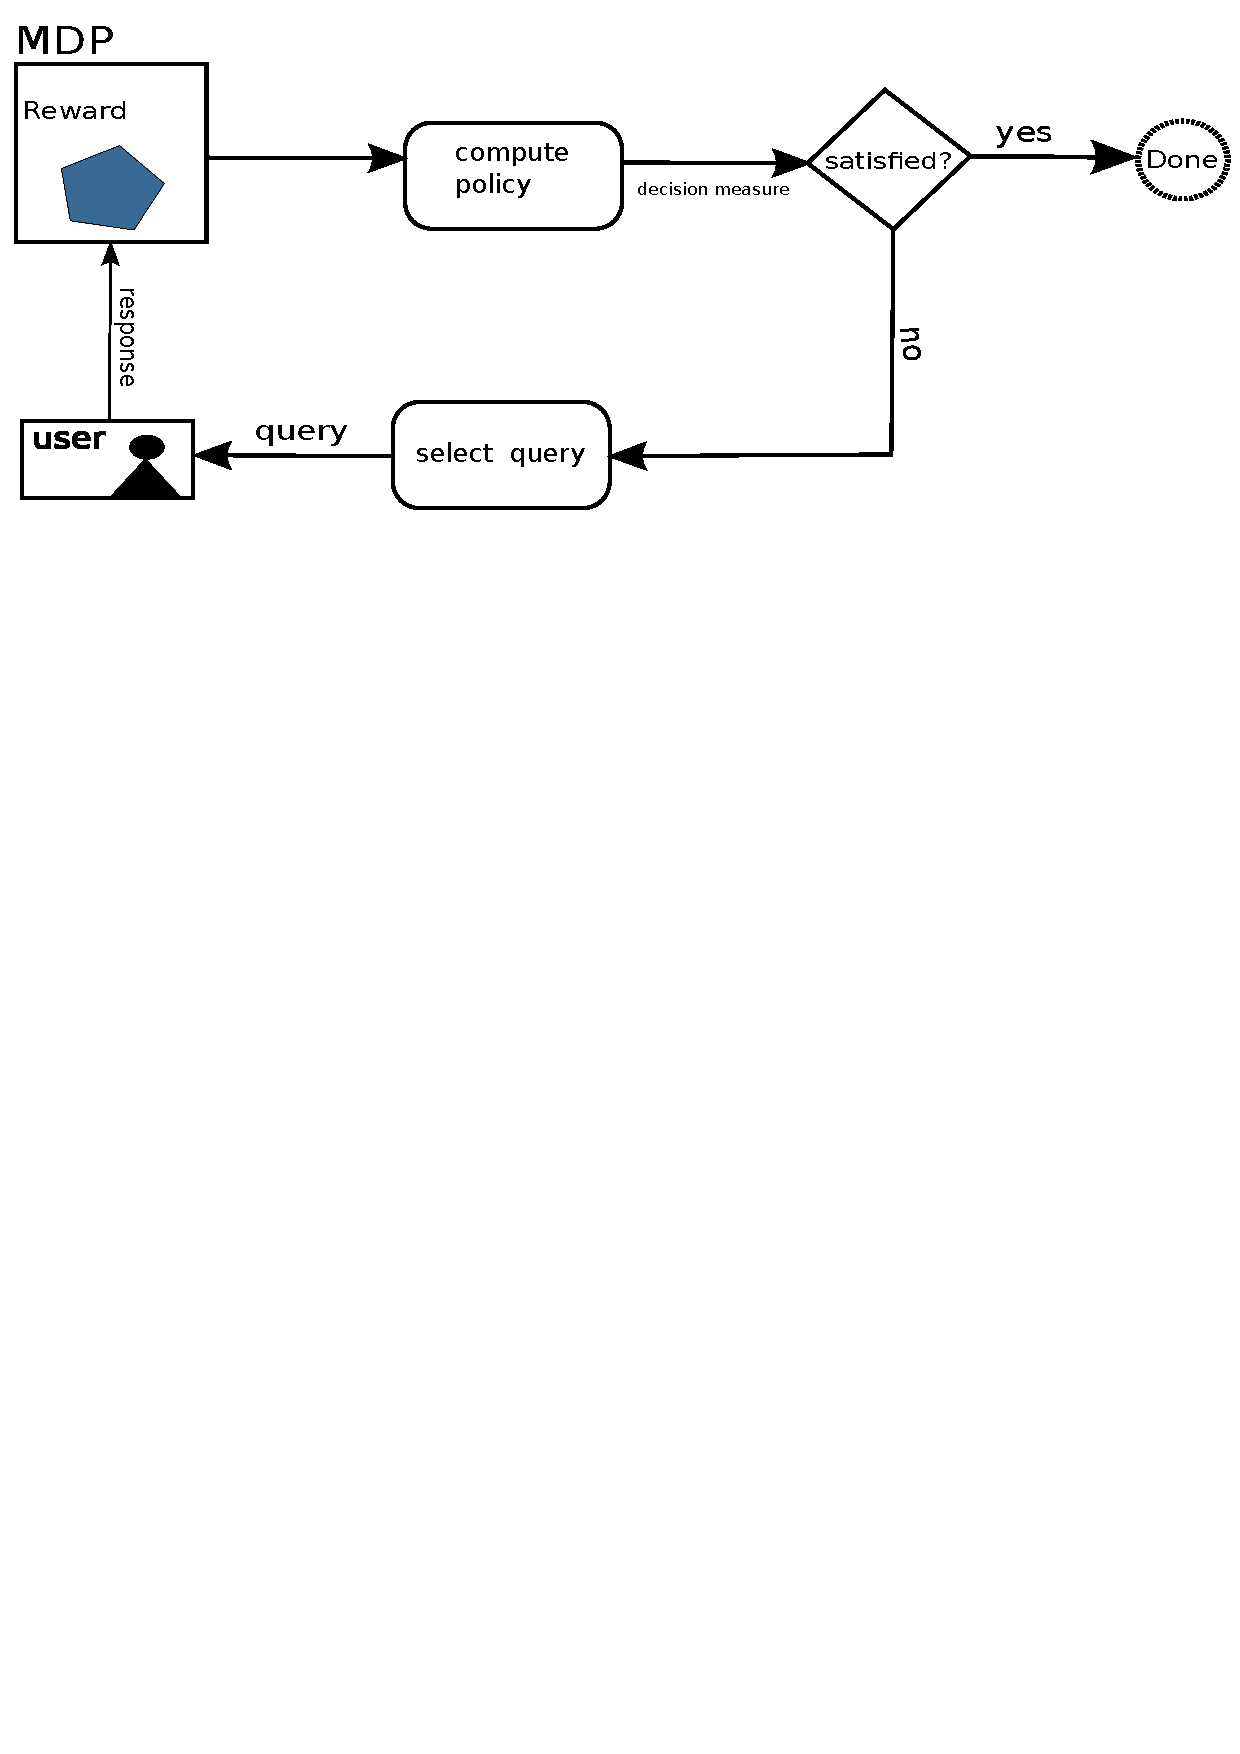
\includegraphics[width = 0.85\textwidth]{images/process+.pdf}};
\node [align=left] at (-118pt,161pt){$\Lambda$};
\end{tikzpicture}    
\end{figure}

\end{frame}

%%%%%%%%%%%%%%%%%%%%%%%%%%%%%%%%%%%
\begin{frame}{What is Advantage}
\begin{block}{}
\remark{Advantage} of pair $(s,a)$ is:
$\bar{A}(s, a) = \bar{Q}(s, a) - \bar{V}(s)$
\end{block}

\centering
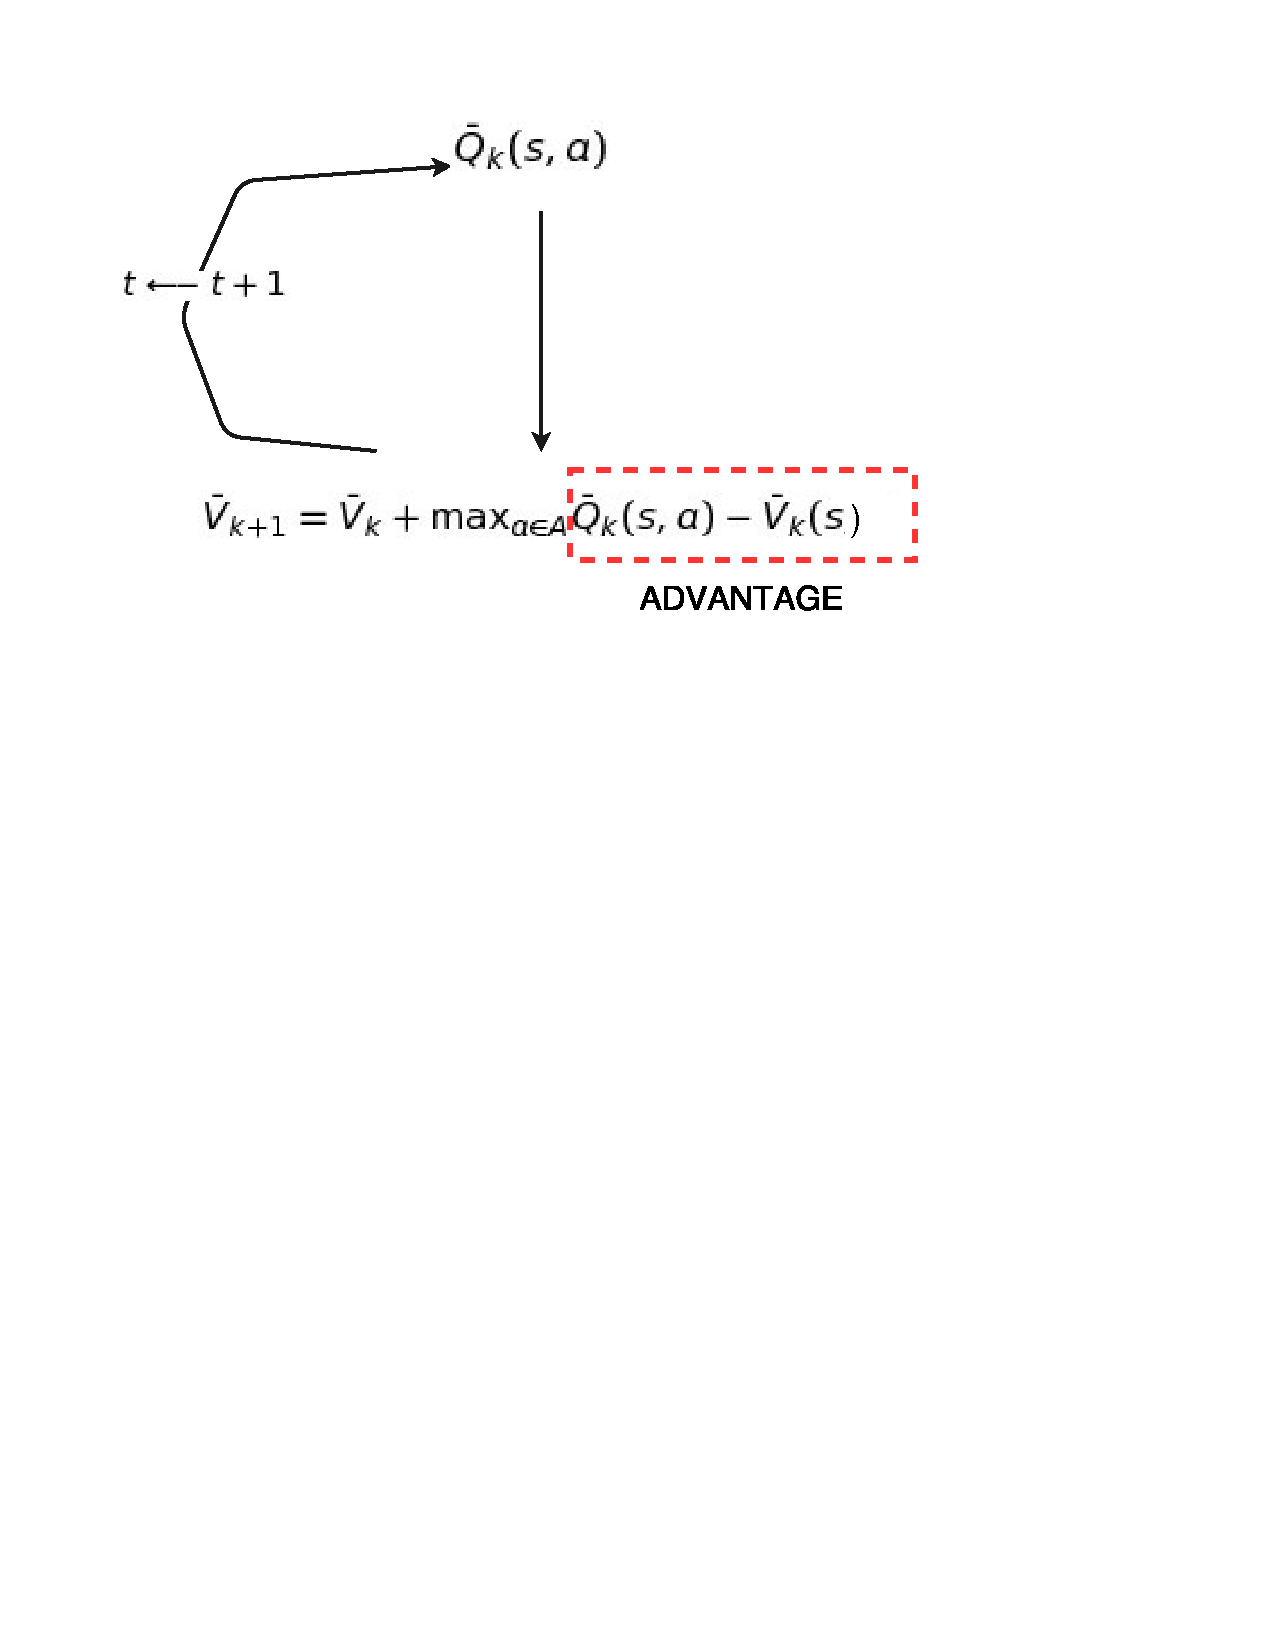
\includegraphics[scale=0.4]{figures-new/advantage}

\end{frame}
%%%%%%%%%%%%%%%%%%%%%%%%%%%%%%%%%%%%%%%%%%%%%

\begin{frame}
\begin{center}

Advantage Based Value Iteration algorithm (ABVI) ~\\
{\color{red} Elicitation}

\end{center}
\end{frame}

%%%%%%%%%%%%%%%%%%%%%%%%%%%%%%%%%%%%%
\begin{frame}[plain]
{Advantage Based Value Iteration algorithm}
\Fontvi
\begin{columns}
\begin{column}{.48\textwidth}
\textbf{IVI Algorithm}: ~\\
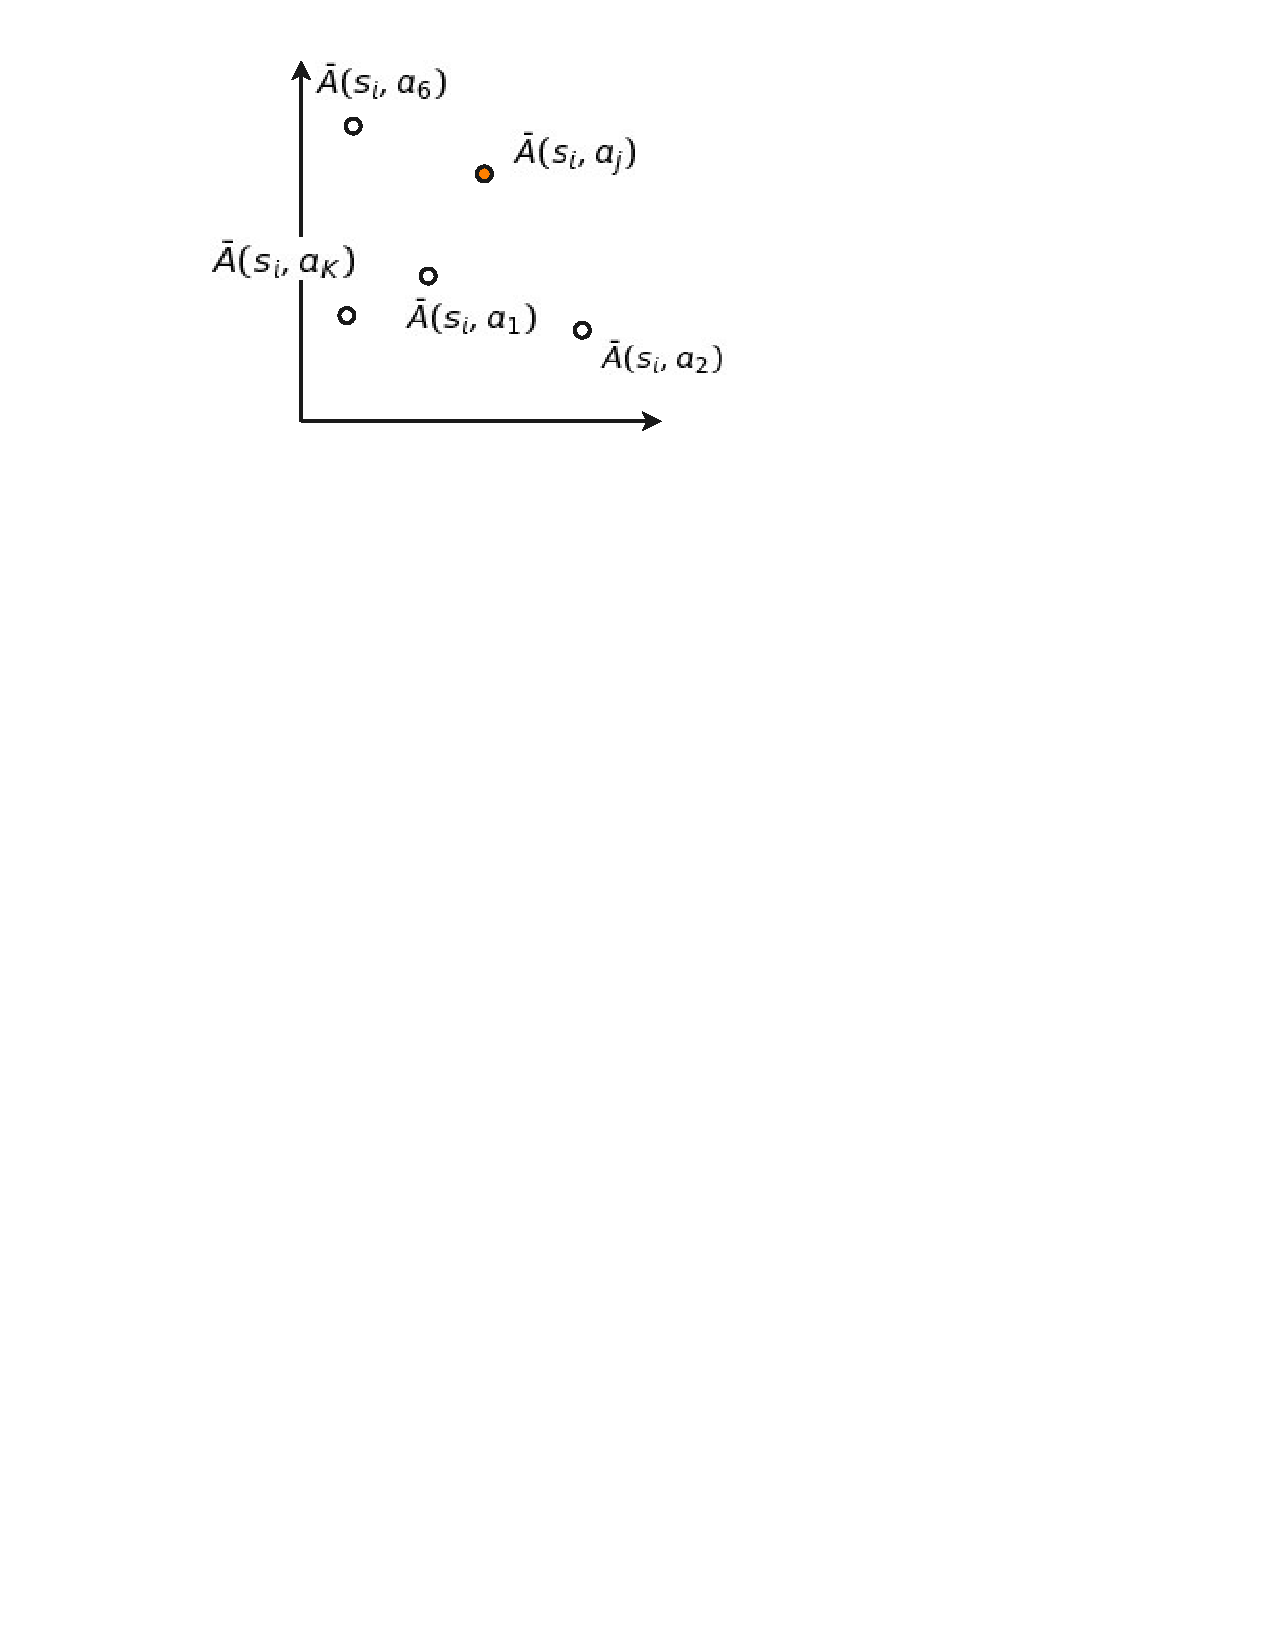
\includegraphics[width = 0.7\textwidth]{figures-new/adv-tree} ~\\
Compare two policies with {\color{red} only one} pair $(s,a)$ difference: ~\\
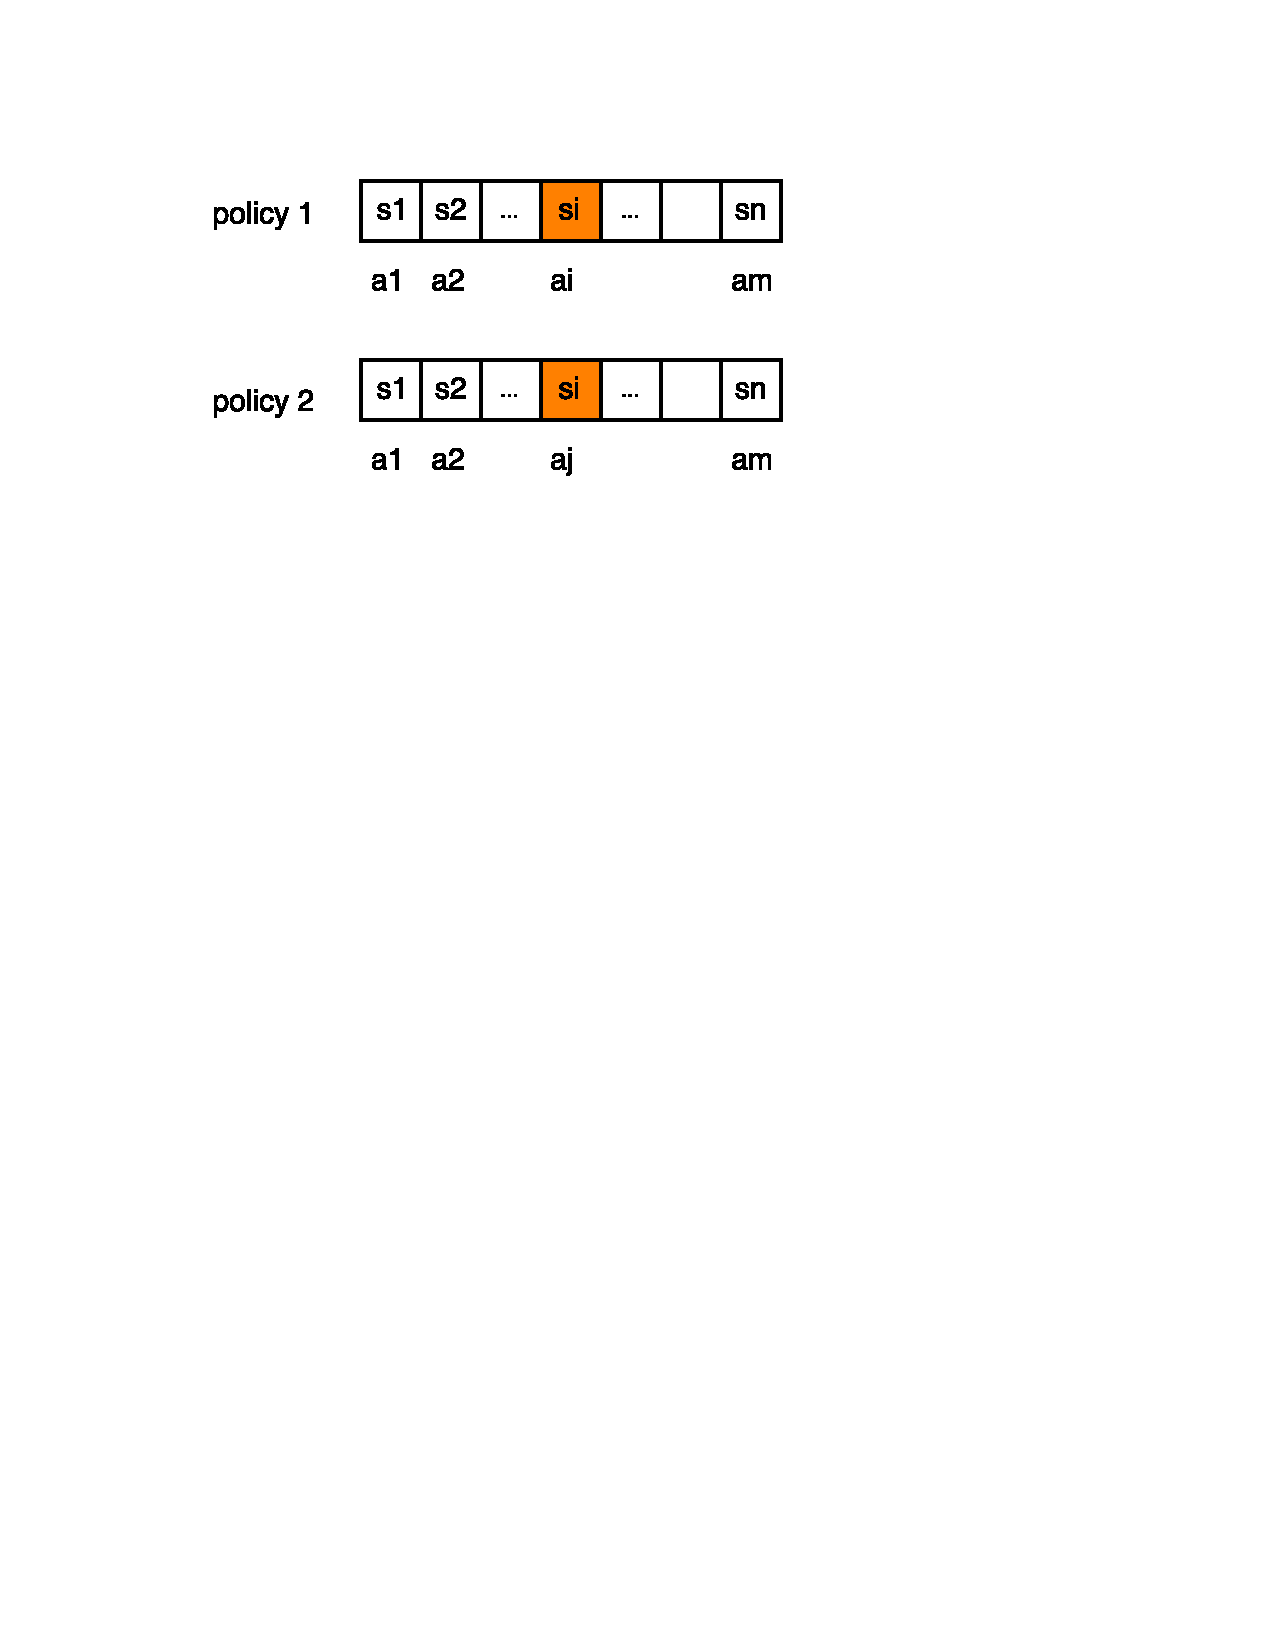
\includegraphics[width = 0.9\textwidth]{figures-new/improv} ~\\
{\color{red} DRAWBACK}: some vector comparisons proposed to the user do not add new information on user preferences.
\end{column}
\hfill
\begin{column}{.48\textwidth}
\textbf{ABVI algorithm}: ~\\
{\color{red} IDEA}: generate more informative queries by clustering advantages.
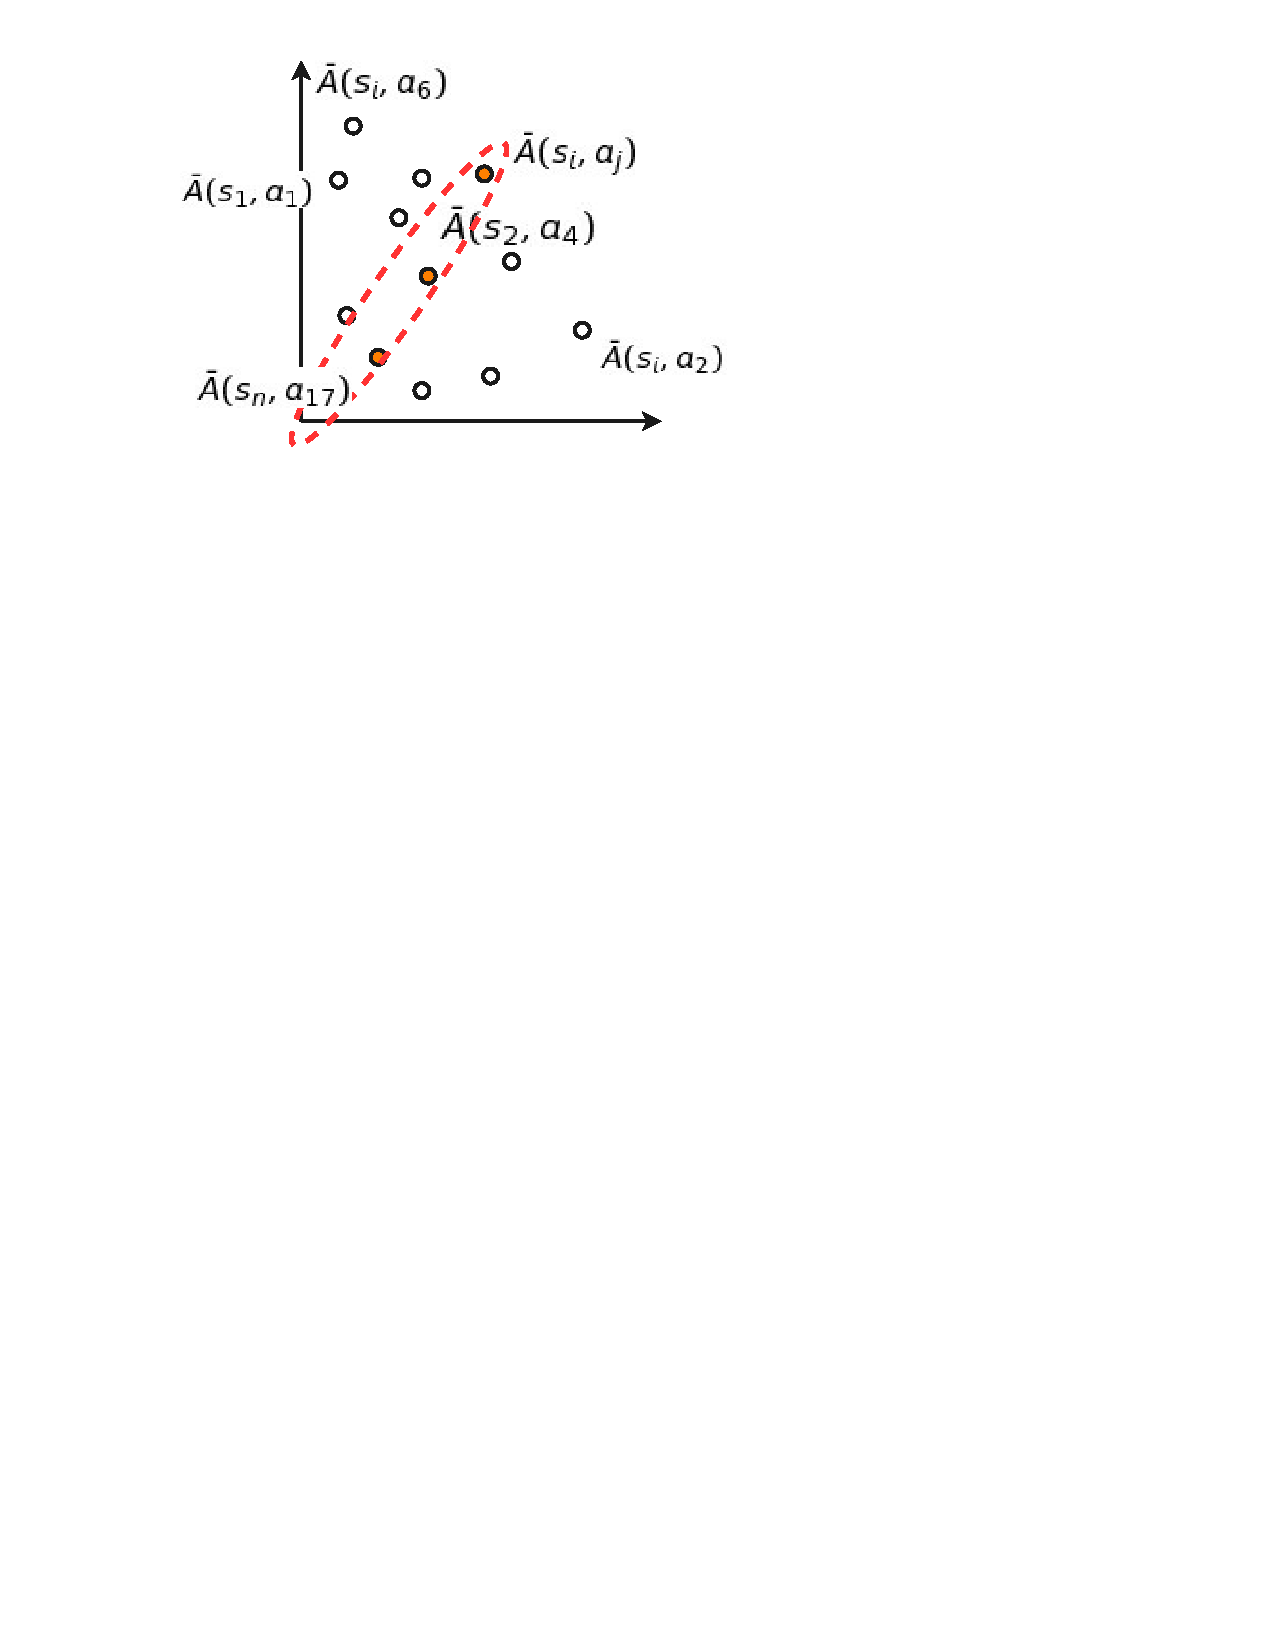
\includegraphics[width = 1.1\textwidth]{figures-new/improv-with-cluster}  ~\\
Instead we compare two policies with {\color{red}  several} different state/action pairs difference ~\\
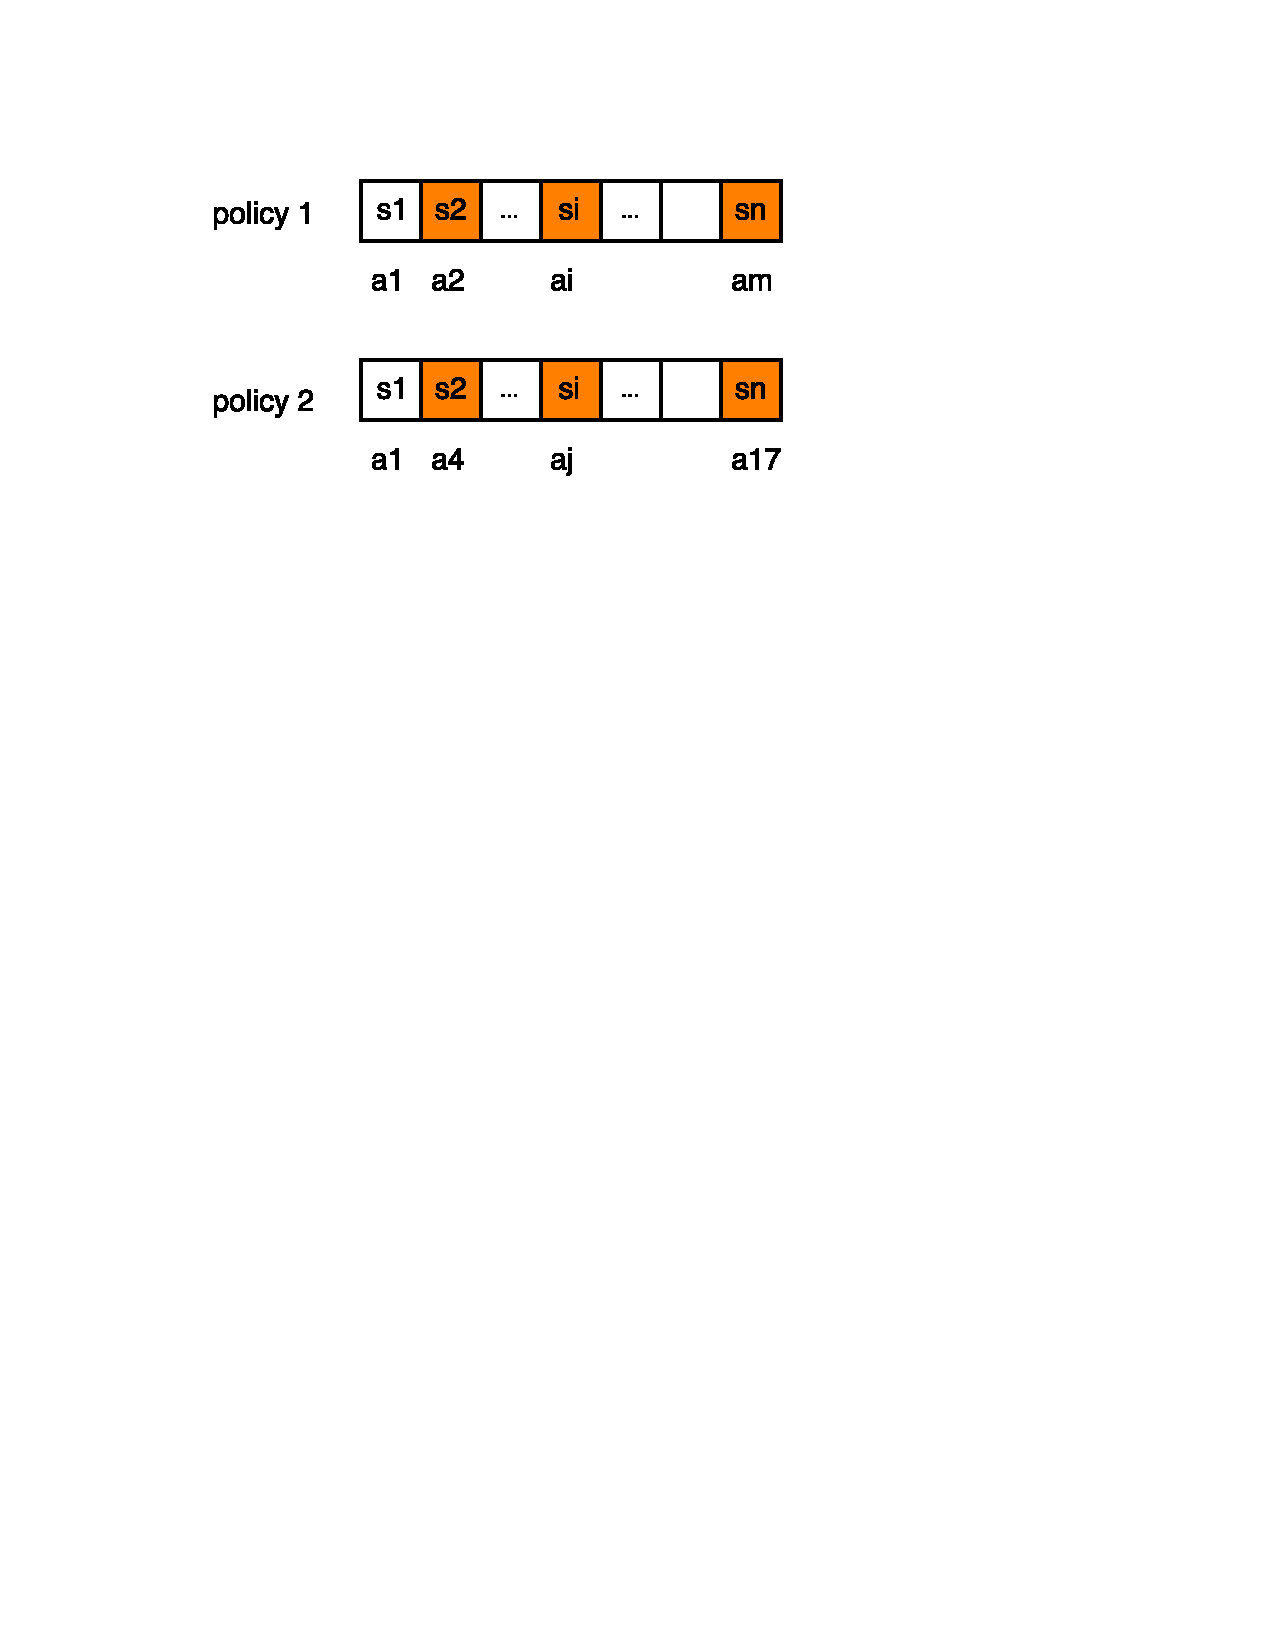
\includegraphics[width = 0.7\textwidth]{figures-new/improv-cluster}
 
\end{column}
\end{columns}

\only<2>{
\begin{textblock*}{80mm}(22mm,0.25\textheight)
\begin{tcolorbox}[colback=green!5,colframe=green!40!black]{ABVI algorithm:}

\begin{itemize}
\item[] $\bar{V}_t$ is given
\item[] for all $s$ and $a$
	\begin{itemize}
	\item[] compute all $|S|\times |A|$ advantages
	\item[] \textbf{cluster the advantages}
	\end{itemize}
\item[] $\bar{V}_{\text{best}} \longleftarrow (0, \cdots 0)$
\item[] for each cluster 
	\begin{itemize}
	\item $\bar{V}_{t+1} \longleftarrow$ getBest($\bar{V}_{\text{best}}$, $\bar{V}_t+$ sum of advantages in cluster )
	\end{itemize}

\end{itemize}

\end{tcolorbox}
\end{textblock*}
}

\end{frame}
%%%%%%%%%%%%%%%%%%%%%%%%%%%%%%%%%%%%%%%%%%%%%%%%%%%%%%%%%%%%%%%%%%%%%%%%%

%%%%%%%%%%%%%%%%%%%%%%%%%%%%%%%%%%%%%%%%%%%%%%%%%%%%%%%%%%%%%%%%%%%%%%%%%
\begin{frame}{Results for confident Users}

\only<1,2,3>{
Random MDPs with $256$ states, $5$ actions and different number of objectives $d=4,5,6$.% for  {\color{red} confident users}
}

\only<1>{
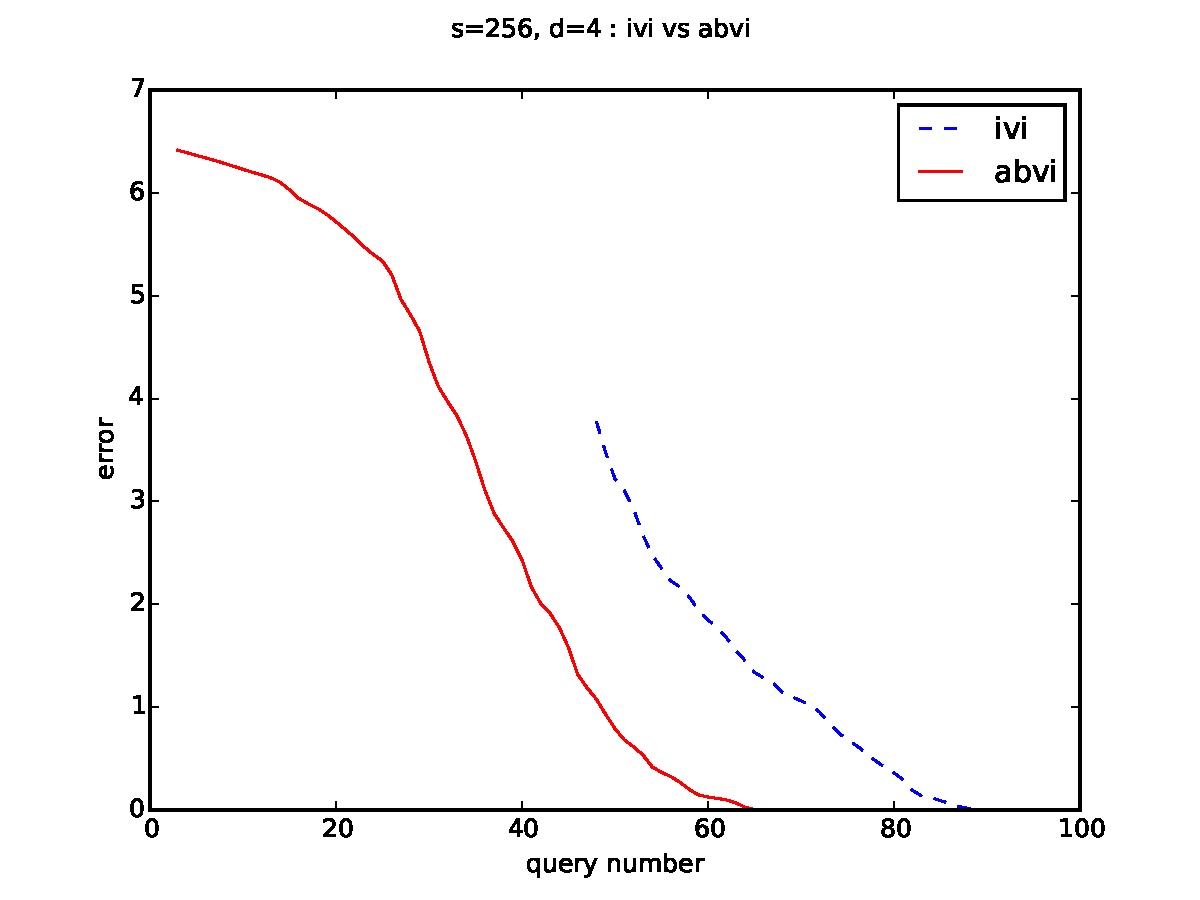
\includegraphics[width=0.8\textwidth]{s256/s-256-d-4.pdf}
}

\only<2>{
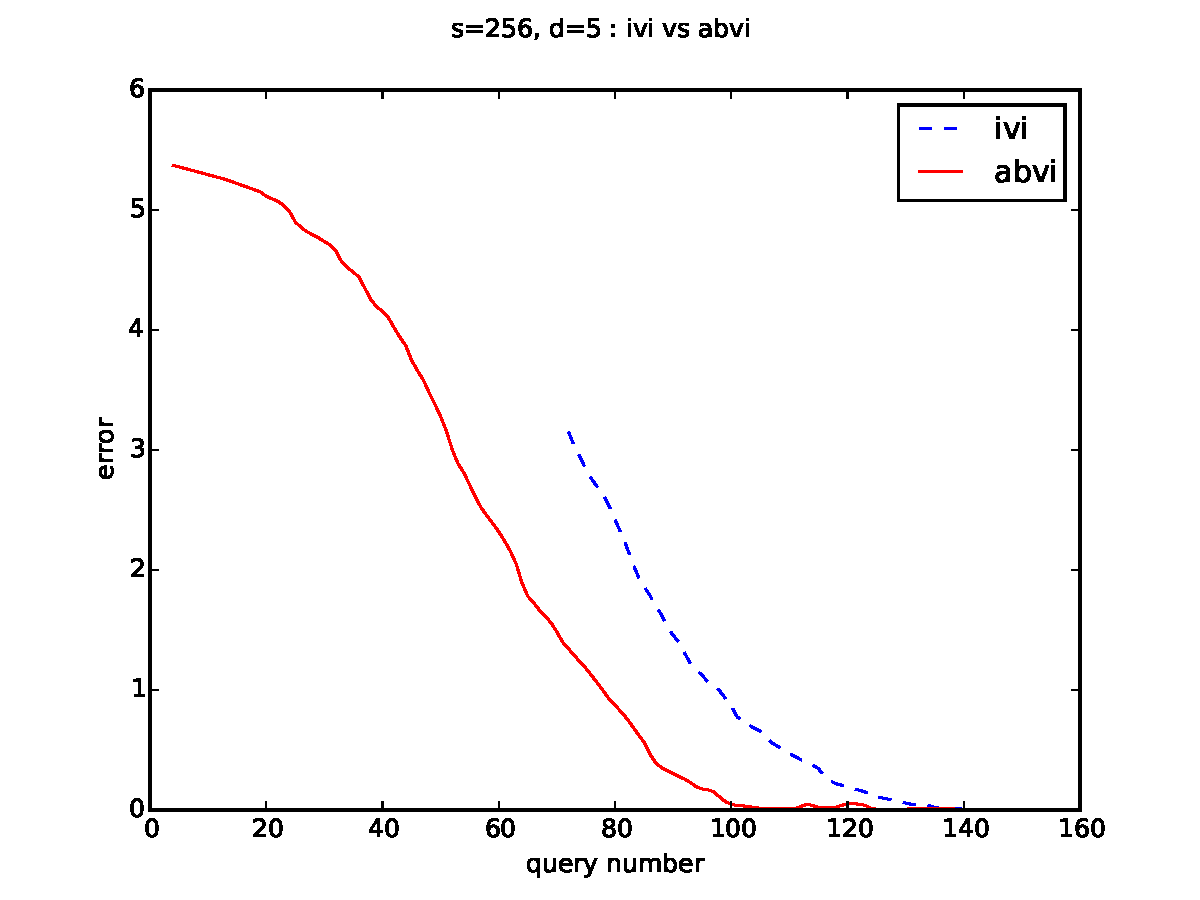
\includegraphics[width=0.8\textwidth]{s256/s-256-d-5.pdf}
}

\only<3>{
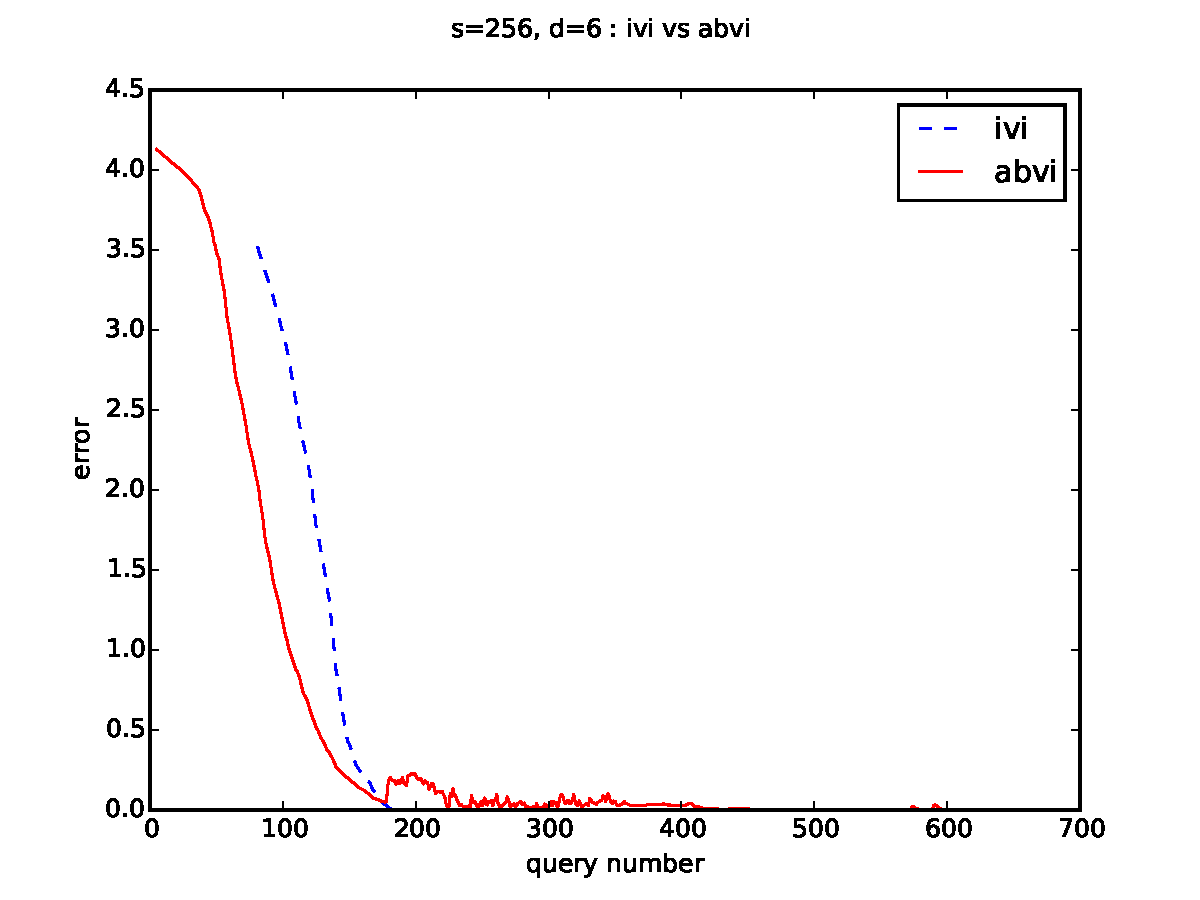
\includegraphics[width=0.8\textwidth]{s256/s-256-d-6.pdf}
}
\end{frame}

%%%%%%%%%%%%%%%%%

\begin{frame}[plain]{Results with Noisy Answers}
\only<1,2,3,4>{
The results on $128$ states, $5$ actions and $d=4$ objectives for different noise parameters: $0.001, 0.01, 0.1$ and with out noise are:

}
\only<1>{
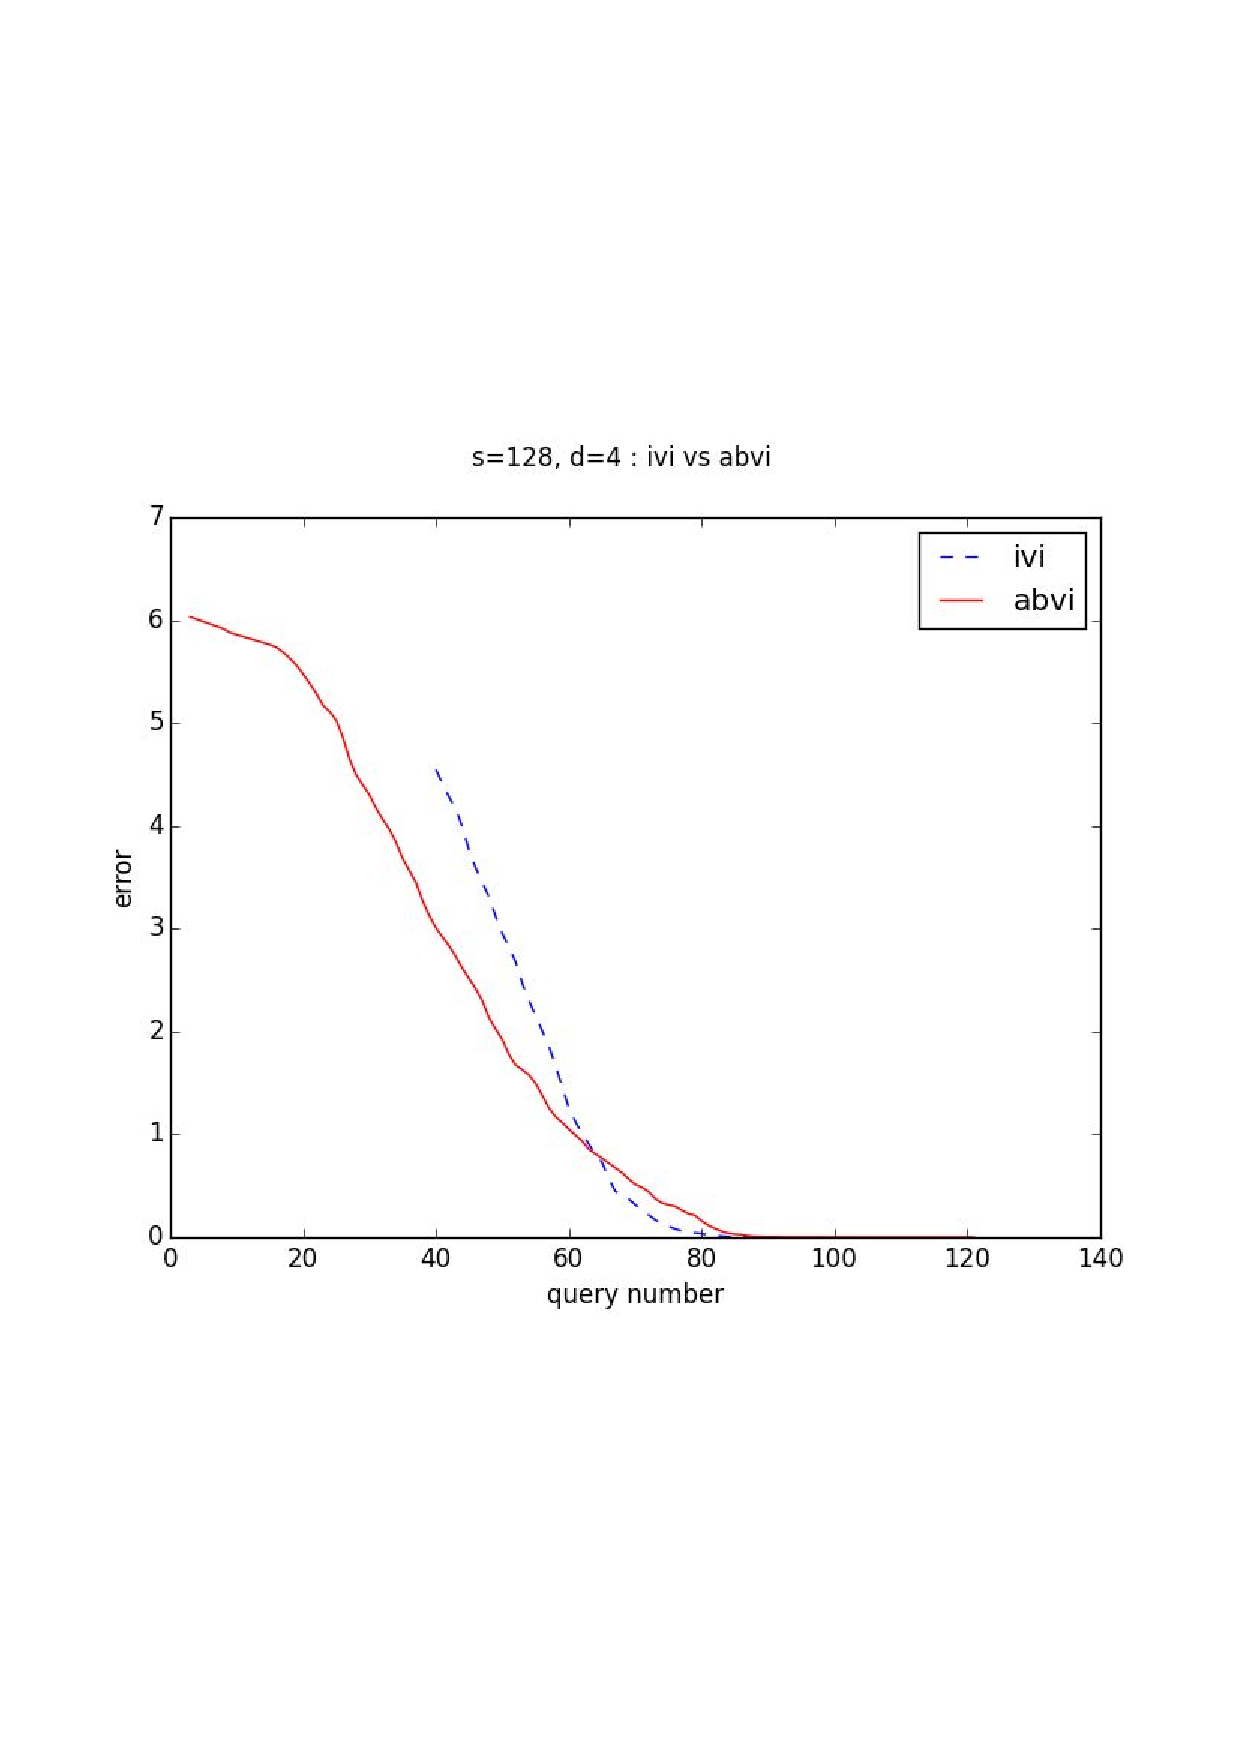
\includegraphics[width=0.8\textwidth]{s-128-d-4-noisy/d-4.pdf}
}

\only<2>{
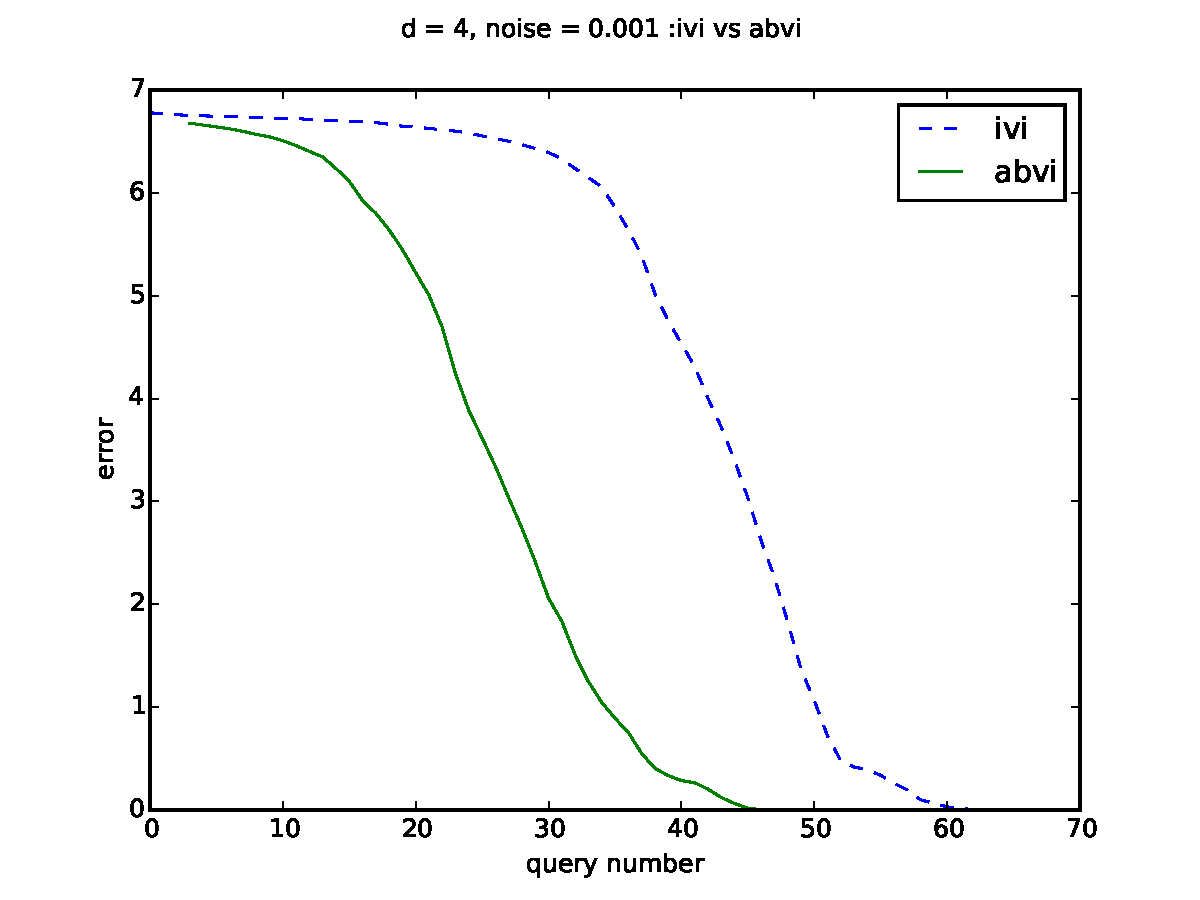
\includegraphics[width=0.8\textwidth]{s-128-d-4-noisy/result0-001.pdf}
}

\only<3>{
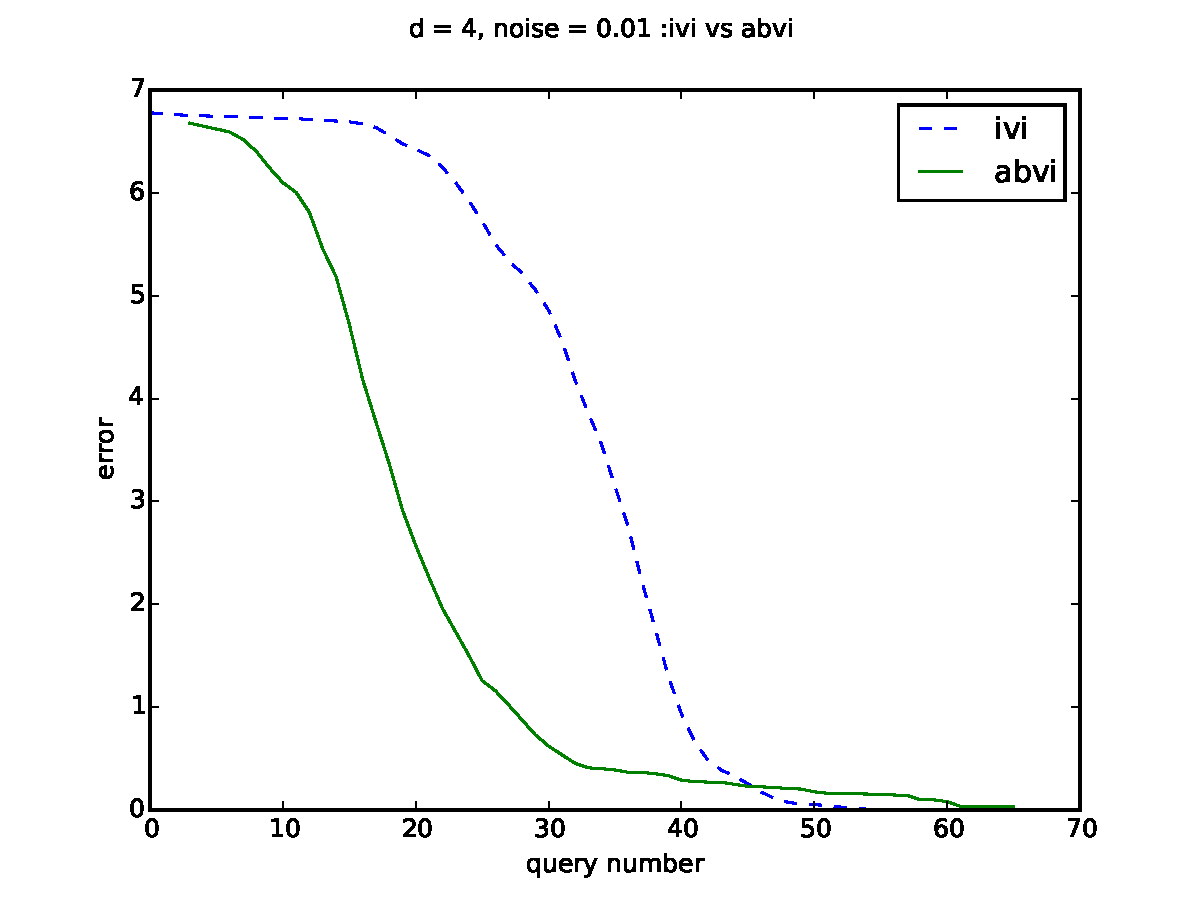
\includegraphics[width=0.8\textwidth]{s-128-d-4-noisy/result0-01.pdf}
}

\only<4>{
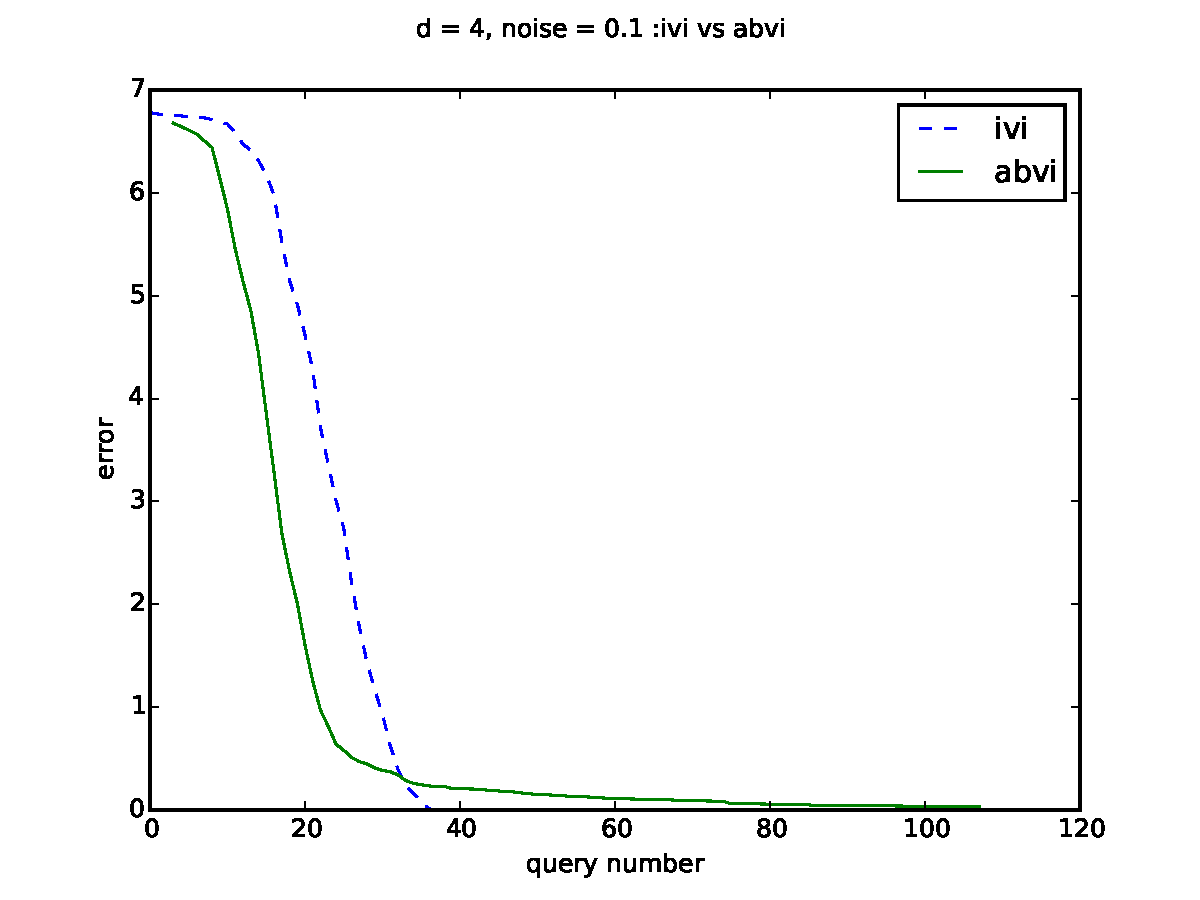
\includegraphics[width=0.8\textwidth]{s-128-d-4-noisy/result0-1.pdf}
}

\end{frame}

%%%%%%%%%%%%%%%%%%%%
\begin{frame}{Conclusion}

\remark{ Advantage based Value Iteration}
\begin{itemize}
\item the \textbf{clustering phase} in the advantage based value iteration algorithm allows a \textbf{speed up} in comparison to the value iteration method.
\item the advantage based value iteration algorithm is \textbf{more robust w.r.t uncertain users} than the IVI algorithm.
%\item {\color{red} we wish to:} speed up its convergence at the end of the algorithm. 
\end{itemize}

\end{frame}

%%%%%%%%%%%%%%%%%%%%%%%%%%%
\begin{frame}
\begin{center}
	\textbf{propagation-search algorithm}
	\alert{Elicitation}
\end{center}
\end{frame}

%%%%%%%%%%%%%%%%%%%%%%%%%%% 
\Fontvi
\begin{frame}
In Propagation-search algorithm, \textbf{instead of querying the users immediately}
\begin{itemize}
\item first we compute all the queries offline
\item second we find the optimal policy by proposing some of them to the user 
\end{itemize}
  
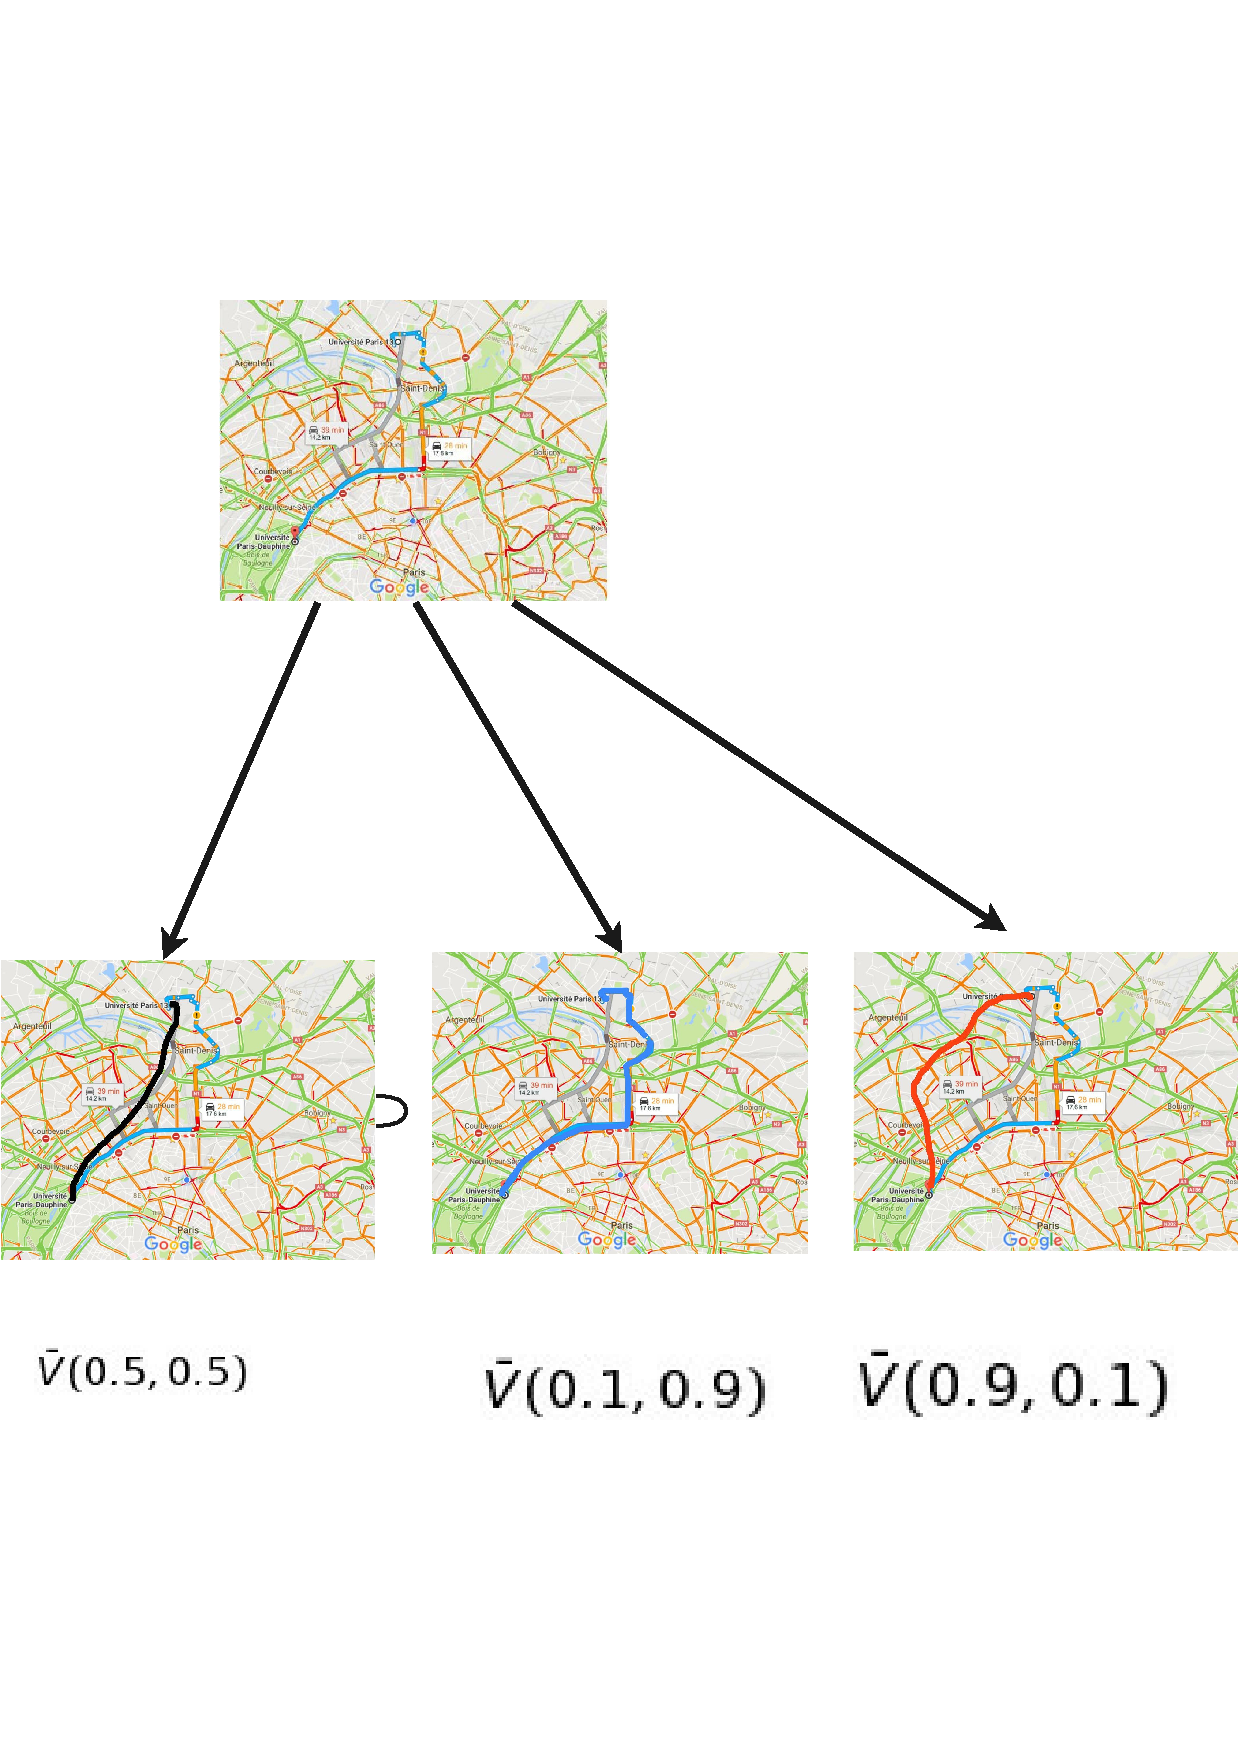
\includegraphics[width=0.5\textwidth]{figures-new/pro} 
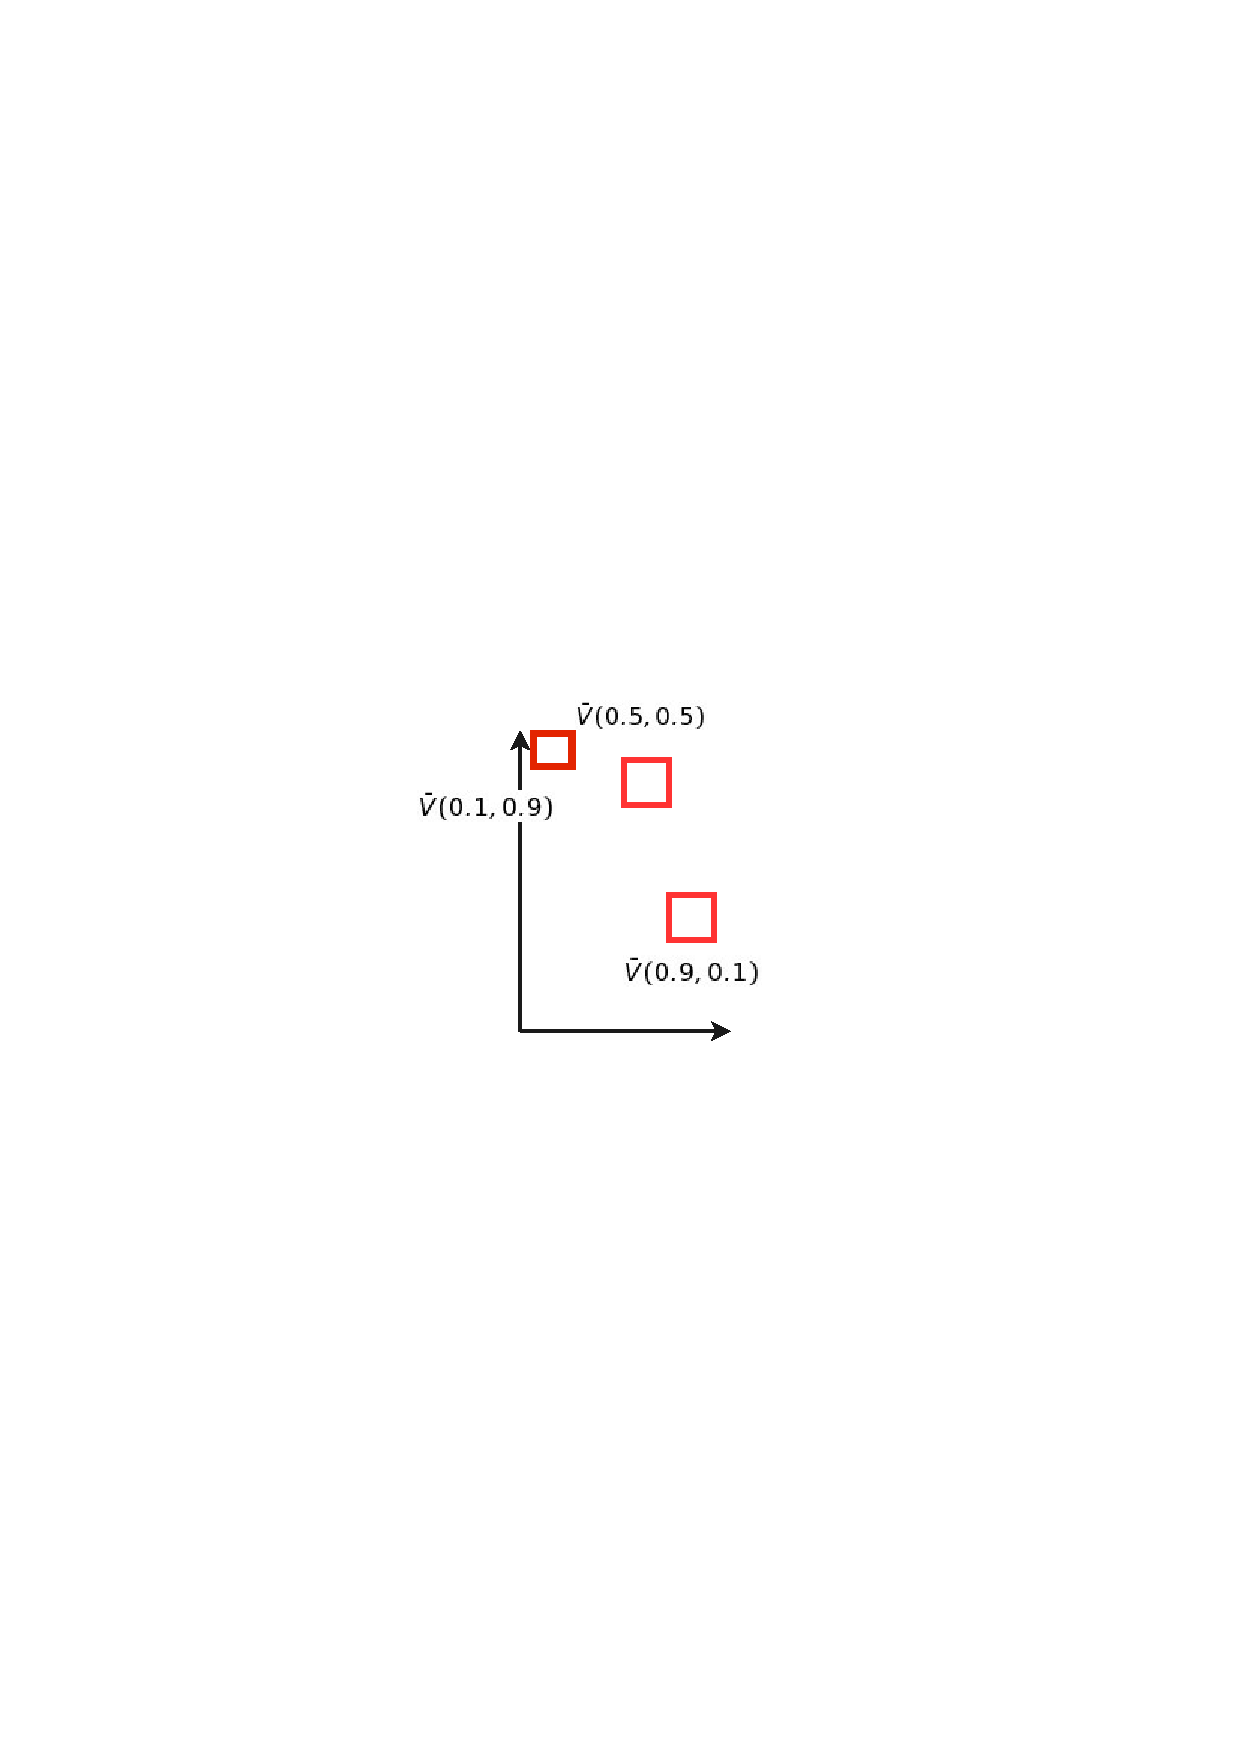
\includegraphics[width=0.5\textwidth]{figures-new/search} ~\\
\begin{columns}
\begin{column}{0.48\textwidth}
These queries are generated from the set of nondominated vectors.
\end{column}
\hfill
\begin{column}{0.48\textwidth}
By querying a few pairs to the user, we find the optimal policy respecting his preferences. 
\end{column}
\end{columns}
\end{frame}

%%%%%%%%%%%%%%%%%%%%%%%%%%%%%%%%%%%%%%%%%%%%%%%%%%%%%%
\begin{frame}{Propagation Algorithm}
%\Fontvi
\begin{columns}

\begin{column}{.48\textwidth}
The basic idea is to search using \alert{Breadth-first search}: ~\\
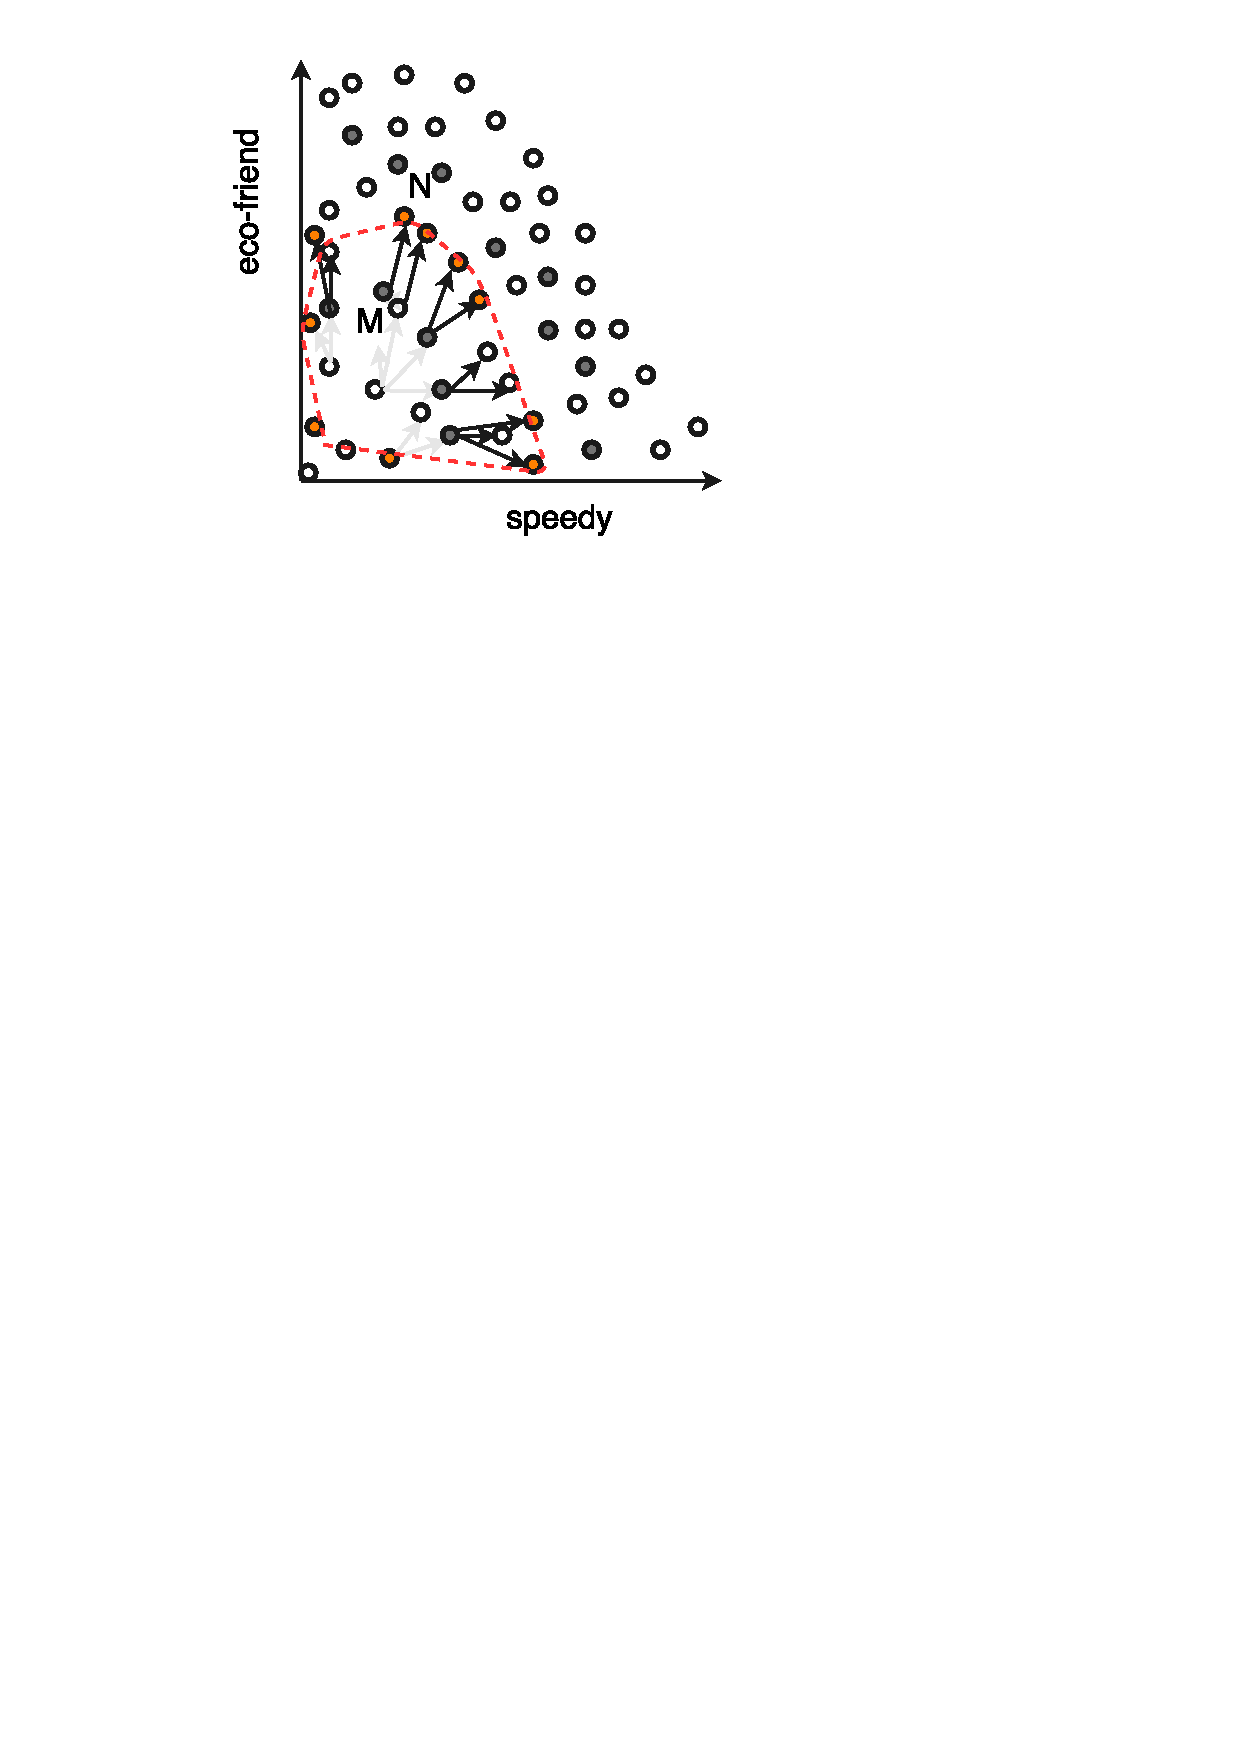
\includegraphics[width=0.7\textwidth]{figures-new/domin-normal} ~\\
The explored vectors improves {\color{red}Advantage by Advantage}: $\bar{V}^{\pi}_N = \bar{V}^{\pi}_M + \bar{A}(s,a) $

\end{column}
\hfill
\begin{column}{.48\textwidth}
To compute more useful $\bar{V}$s and save less number of vectors, we {\color{red}cluster advantages}: ~\\
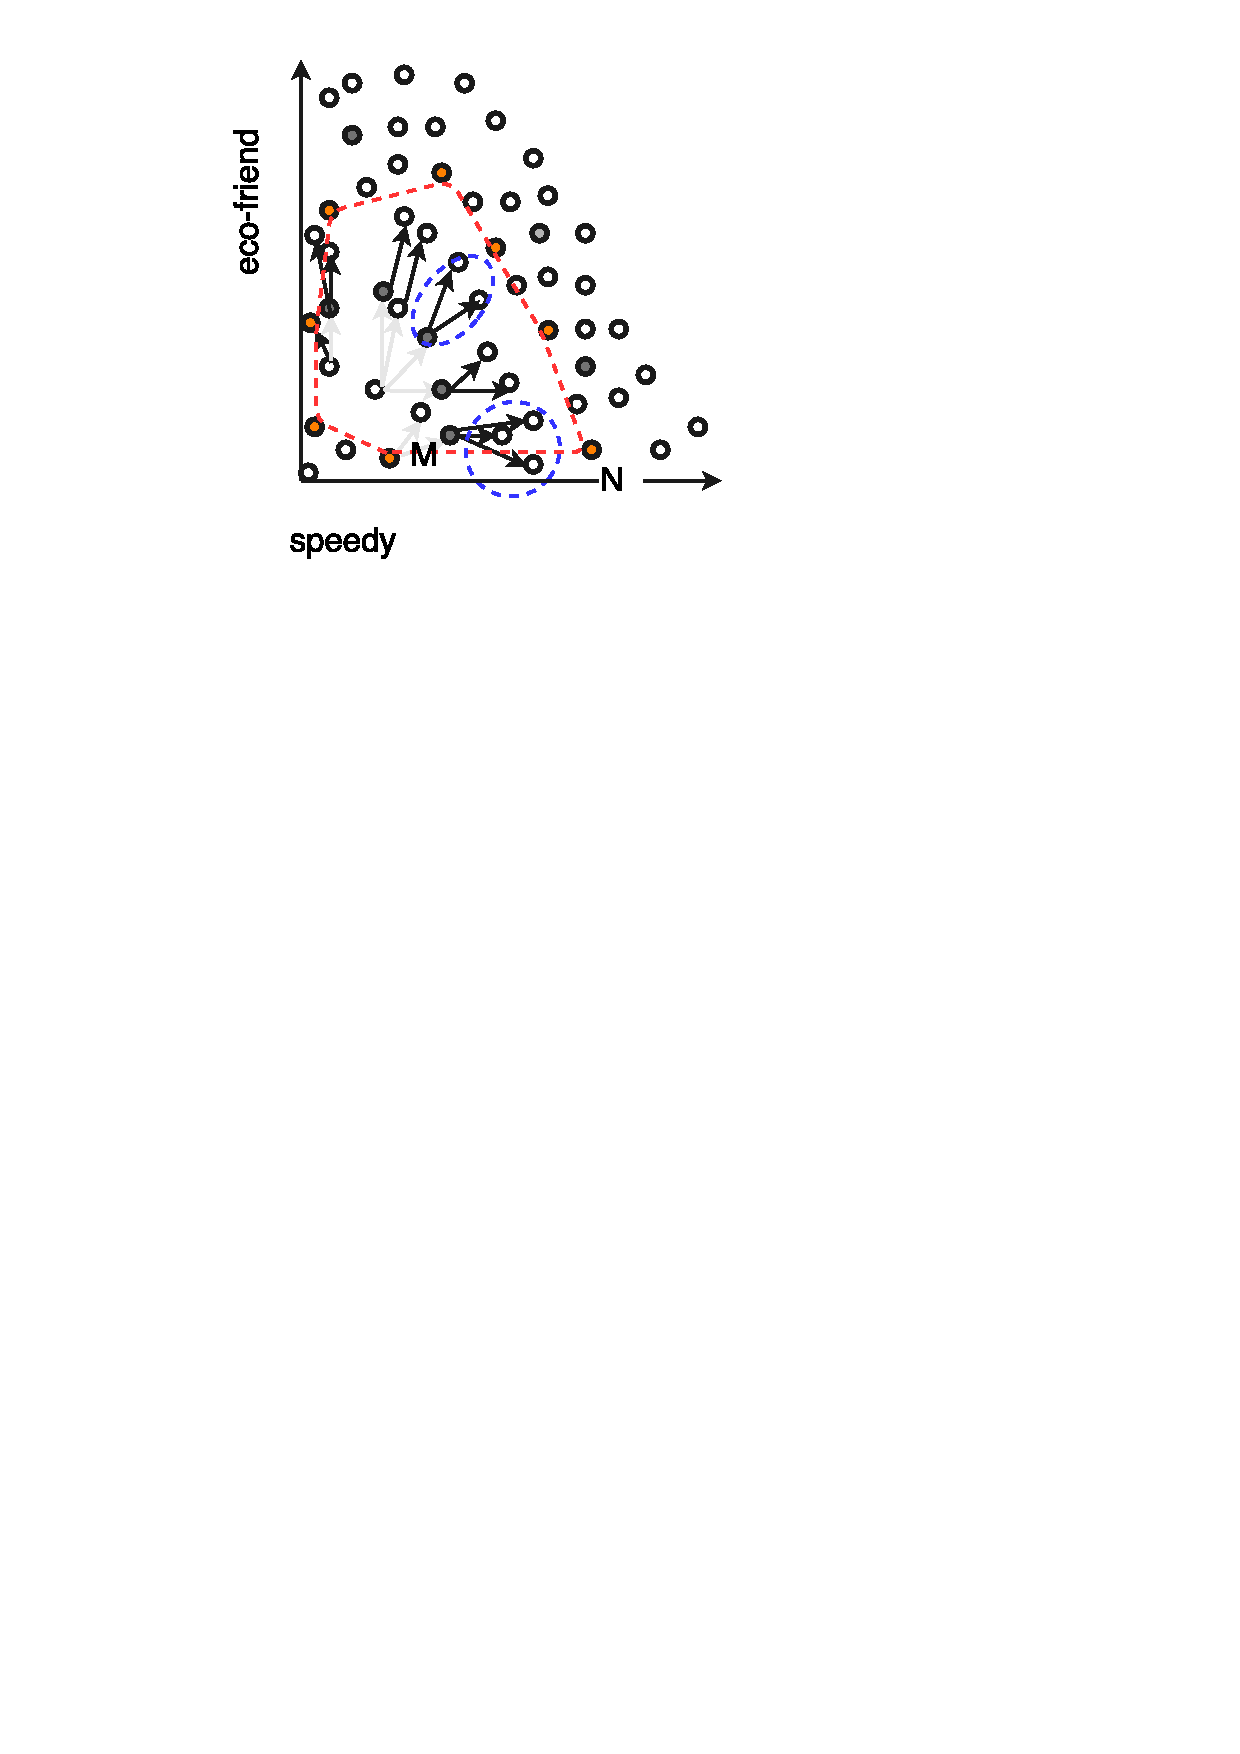
\includegraphics[width=0.7\textwidth]{figures-new/imp-clust} ~\\
$\bar{V}^{\pi}_N = \bar{V}^{\pi}_M + \bar{A}(s,a)+ \bar{A}(s',a')+ \bar{A}(s'',a'')$
\end{column}

\end{columns}
\pause 
\only<2>{
\begin{textblock*}{80mm}(22mm,0.25\textheight)
\begin{tcolorbox}[colback=green!5,colframe=green!40!black]{Algorithm}

\begin{itemize}
\item $\mathcal{V} \longleftarrow \bar{V}_1, \cdots,  \bar{V}_d$ \small{policy values of extreme users}
\item Repeat
\begin{itemize}
%\item for each $\bar{V} \in \mathcal{V}$
	%\begin{itemize}
	\item \textbf{expand} $\mathcal{V}$ using \textbf{clustering advantages} 
	\item \textbf{make a convex} hull on the union of $\mathcal{V}$ an expanded vectors
	%\end{itemize}
\end{itemize}
\item Until convergence
\end{itemize}
%\center
%{\color{red}$|\mathcal{V}| \sim (\frac{1}{\epsilon^d})$}
\end{tcolorbox}
\end{textblock*} 
}
\end{frame}

%%%%%%%%%%%%%%%%%%%%%%%%%%%%%%%%%%%%%%%%%%%%%%%%%%%%%%
\begin{frame}{Search the optimal policy satisfying the user}


%Idea: Pairwise comparison using three ordered comparisons: $1$- Pareto, $2$- Kdominance, $3$- query user

%\begin{columns}
%\begin{column}{.48\textwidth}
{\small 
\begin{itemize}
\item generate minimum set of pairs %: $P = \{ (\bar{V}_i, \bar{V}_j) \in \mathcal{V}^2 \text{ s.t. } i<j \}$
\item Find comparable pairs w.r.t Pareto or Kdominance %$T = \{ (\bar{V}_i, \bar{V}_j) \in P  \text{ s.t. } \text{they are comparable}\}$
\item while there exists a set of not comparable pairs

	\begin{itemize}
	{\small
	\item Choose the Halve-largest-gap pair from set of not comparable pairs
	\item Ask the pair to the user
	}
	\end{itemize}
		
\end{itemize}
}
%\end{column}
%\hfill
%\begin{column}{.48\textwidth}
Halve-largest-gap pair : $Pr_{\bar{\lambda} \in \Lambda} [\bar{\lambda} \cdot \bar{V}^{\pi} \geq \bar{\lambda} \cdot \bar{V}^{\pi'}] \simeq \frac{1}{2}$ ~\\

\begin{columns}
\column{.3\textwidth}
\begin{figure}
\centering
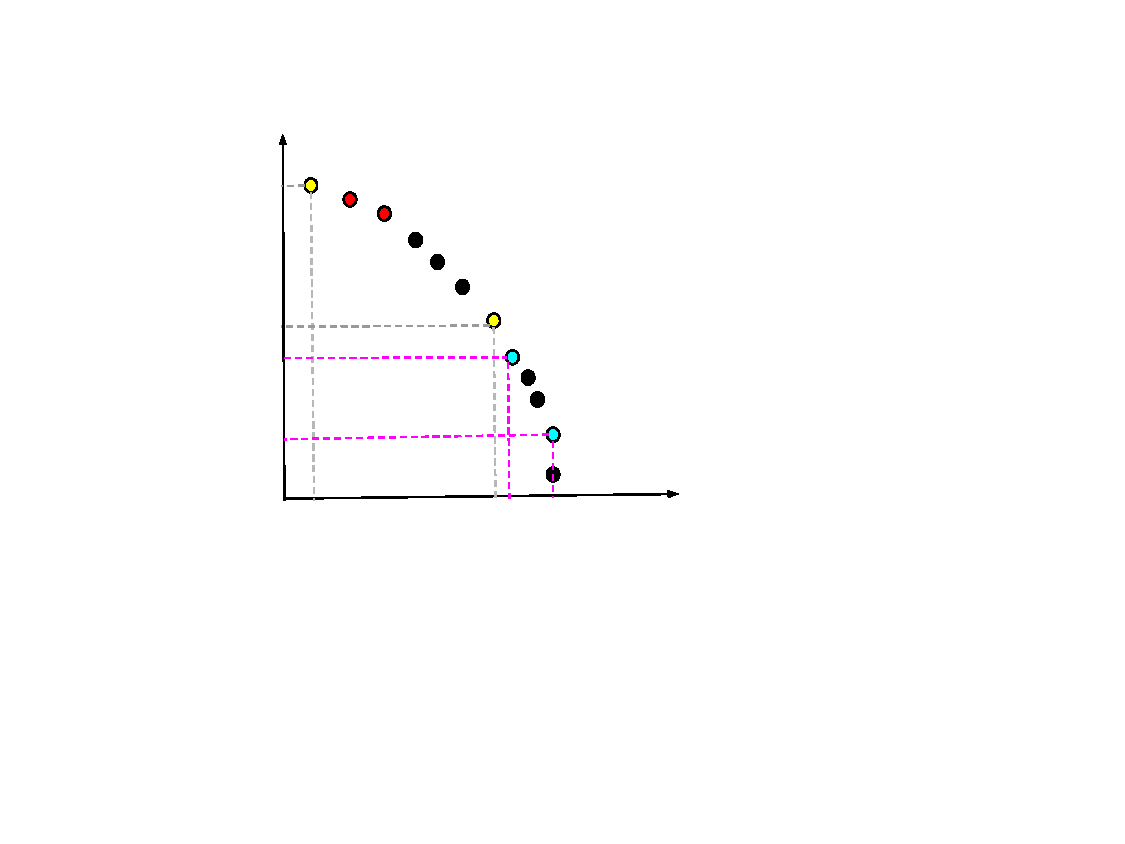
\includegraphics[width=1.\textwidth]{figures/which-pair}
\end{figure}
%
\column{.3\textwidth}
\begin{figure}
\centering
        \begin{tikzpicture}
		\node[] (img) at (-15.5,8.5) {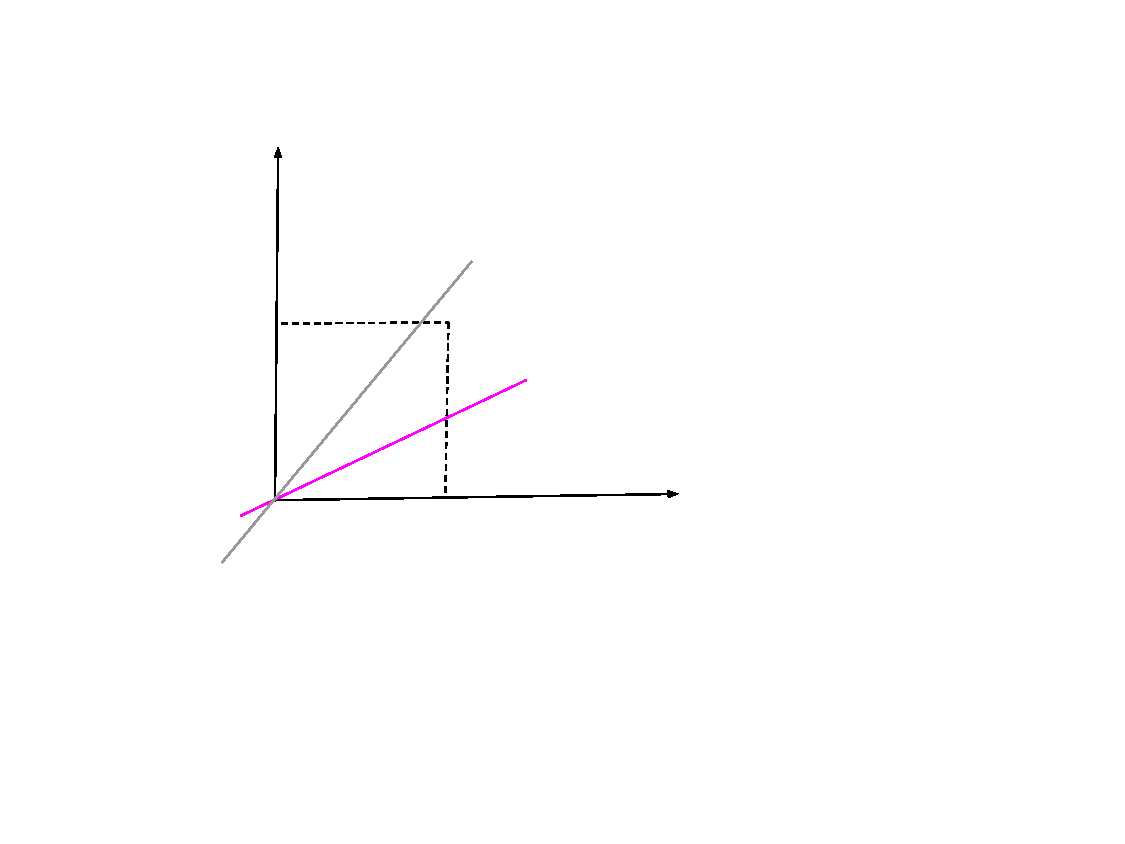
\includegraphics[width=1.\textwidth]{figures/monte-carlo}};
		\node [align=left] at (-16.5, 9.8) {$\lambda_2$};
		\node [align=left] at (-14, 7.4) {$\lambda_1$};
		\end{tikzpicture}
%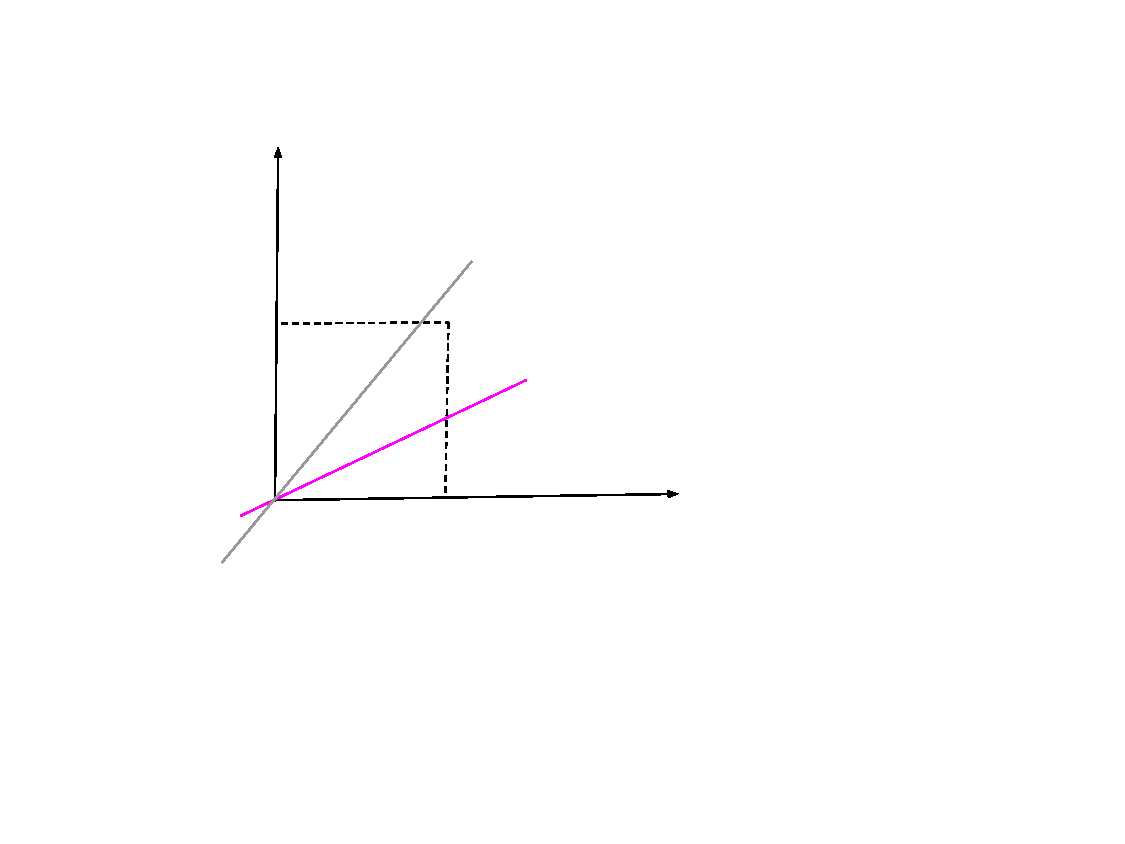
\includegraphics[width=1.\textwidth]{figures/monte-carlo}
%\caption{$\Lambda$ poytope}
\end{figure}
\end{columns}
\centering
{\small the gray cut divides $\Lambda$ into almost two equal parts}
%\end{column}
%\end{columns}
\end{frame}

%%%%%%%%%%%%%%%%%%%%%%%%%%%%%%%%%%%%%%%%%%%%%%%%%%%%%%
\begin{frame}{Results for two simulated random MDPs}
\Fontvi
%Results for two simulated random MDPs: 
%\begin{itemize}
%\item $128$ states, $5$ actions, $d=2,3,4$ and precision of generating optimal policies $0.2$
%\item $128$ states, $5$ actions, $d=2,3,4$ and precision of generating optimal policies $0.1$
%\end{itemize}
%\begin{columns}
%\begin{column}{.48\textwidth}
 
\begin{table}
%\begin{center}
\scalebox{1}{
\begin{tabular}{ | l | l | l | l | l | l | l | }
%\hline
%\multicolumn{6}{ |c| }{Team sheet} \\
\hline
Methods & parameters &$d=2$ & $d=3$ & $d=4$  \\ \hline
\multirow{5}{*}{PSVI} 
 & $|\bar{\mathcal{V}}_{\epsilon}|$ & 8.4 & 43.3 & 4.0  \\
 & Queries & \textbf{3.27}& \textbf{12.05} & \textbf{5.08}  \\  
 & error & 0.00613 & 0.338 & 0.54823 \\
 & propagation time & 33.6377 & 170.1871& 3.036455 \\
 & exploration time & 1.20773   & 36.4435 & 6.022591  \\ \hline
\multirow{3}{*}{IVI } %\footnote{ {\ssmall(Weng $\&$ Zanuttini, 2013)} }} 
 & Queries & 17.38 & 41.16 & 69.18  \\
 & error & \textbf{0.0058} & \textbf{0.319} & \textbf{0.5234}  \\
 & IVI time & 9.8225060   & 5.57657 & 5.30287 \\ \hline\hline
 PSVI & total time & 94.0242 &10501.7171 &304.166 \\ \hline
IVI & total time & 491.1253&278.8285 & 265.1435  \\ \hline
\end{tabular}}
%\end{center}
\end{table}
Average results on $5$ iterations of MDP with $|S|=128$, $|A| = 5$ and $d = 2,3, 4$ with Propagation algorithm accuracy is $\epsilon = 0.2$.
\end{frame}

%%%%%%%%%%%%%%
\begin{frame}

%\end{column}
%\hfill
%\hspace{-0.5cm}
%\begin{column}{.48\textwidth}
\begin{table}
%\begin{center}
\scalebox{1}{
\begin{tabular}{ | l | l | l | l | l | l | l | }
%\hline
%\multicolumn{6}{ |c| }{Team sheet} \\
\hline
Methods & parameters &$d=2$ & $d=3$ & $d=4$  \\ \hline
\multirow{5}{*}{PSVI} 
 & $|\bar{\mathcal{V}}_{\epsilon}|$ & 7.79 & 154.4 & 32.2   \\
 & Queries &  \textbf{2.52}  &   \textbf{15.99}&  \textbf{15.7}  \\  
 & error & 0.0035  & 0.14914 & 0.519   \\
 & propagation time &  57.530  & 3110.348 & 893.4045  \\
 & exploration time & 0.8555 & 229.134 & 95.90481   \\ \hline
\multirow{3}{*}{IVI} 
 & Queries & 17.8 & 42.15& 67.79  \\
 & error & \textbf{0.0033}   &  \textbf{0.142} & \textbf{0.493}   \\
 & IVI time &  10.0345 & 6.99638 & 5.309833  \\ \hline\hline
PSVI & total time & 100.305 & 14567.048&4795.2405 \\ \hline
IVI & total time & 501.725&349.819 &265.49165   \\ \hline
\end{tabular}}
%\end{center}
\end{table}
Average results on $5$ iterations of MDP with $|S|=128$, $|A| = 5$ and $d = 2,3, 4$ with Propagation algorithm accuracy is $\epsilon = 0.1$.
%\end{column}
%\end{columns}

\end{frame}

%%%%%%%%%%%%%%%%%%%%%%%%%%%%%%%%%%%%%%%%%%%%%%%%%%%%%%%

%%%%%%%%%%%%%%%%%%%%%%%%%%%

\begin{frame}
\remark{propagation-search algorithm}
\begin{itemize}
\item the propagation part of the propagation-search algorithm finds \textbf{non-dominated policies for small dimension $d$}

\item in the propagation-search algorithm, a \textbf{clever exploration of the set of non-dominated policies} allows to discover the optimal policy by asking \textbf{less number of queries}. 
\end{itemize}

\end{frame}

%%%%%%%%%%%%%%%%%%%%%%%%%%%
\begin{frame}
\begin{center}
Selected Random Points Method ~\\
{\color{red} Robust Policy}
\end{center}
\end{frame}

%%%%%%%%%%%%%%%%%%%%%%%%%%%%%%%%%%%%%%%%%%%%%%%%%%%%%%
\begin{frame}{Selected Random Points Method for computing minimax regret}
\Fontvi
\begin{columns}
\begin{column}{.45\textwidth}

\begin{itemize}
\item We are not allowed to ask enough number of queries to the user or
\item the $\Lambda$ polytope at the end of the elicitation process is still big
\end{itemize} 

{\color{red}goal}: Computing the robust policy w.r.t the uncertain set of $\Lambda$ using minimax regret criteria:
\begin{equation*}
\pi^* = \text{argmin}_{\pi} \text{max}_{\bar{\lambda} \in \Lambda} \text{max}_{\pi'} \bar{\lambda} \cdot \bar V^{\pi'} - \bar{\lambda} \cdot \bar V^{\pi}
\end{equation*}
\end{column}
\hfill
\begin{column}{.4\textwidth}
Using \alert{Bender's Decomposition}: ~\\
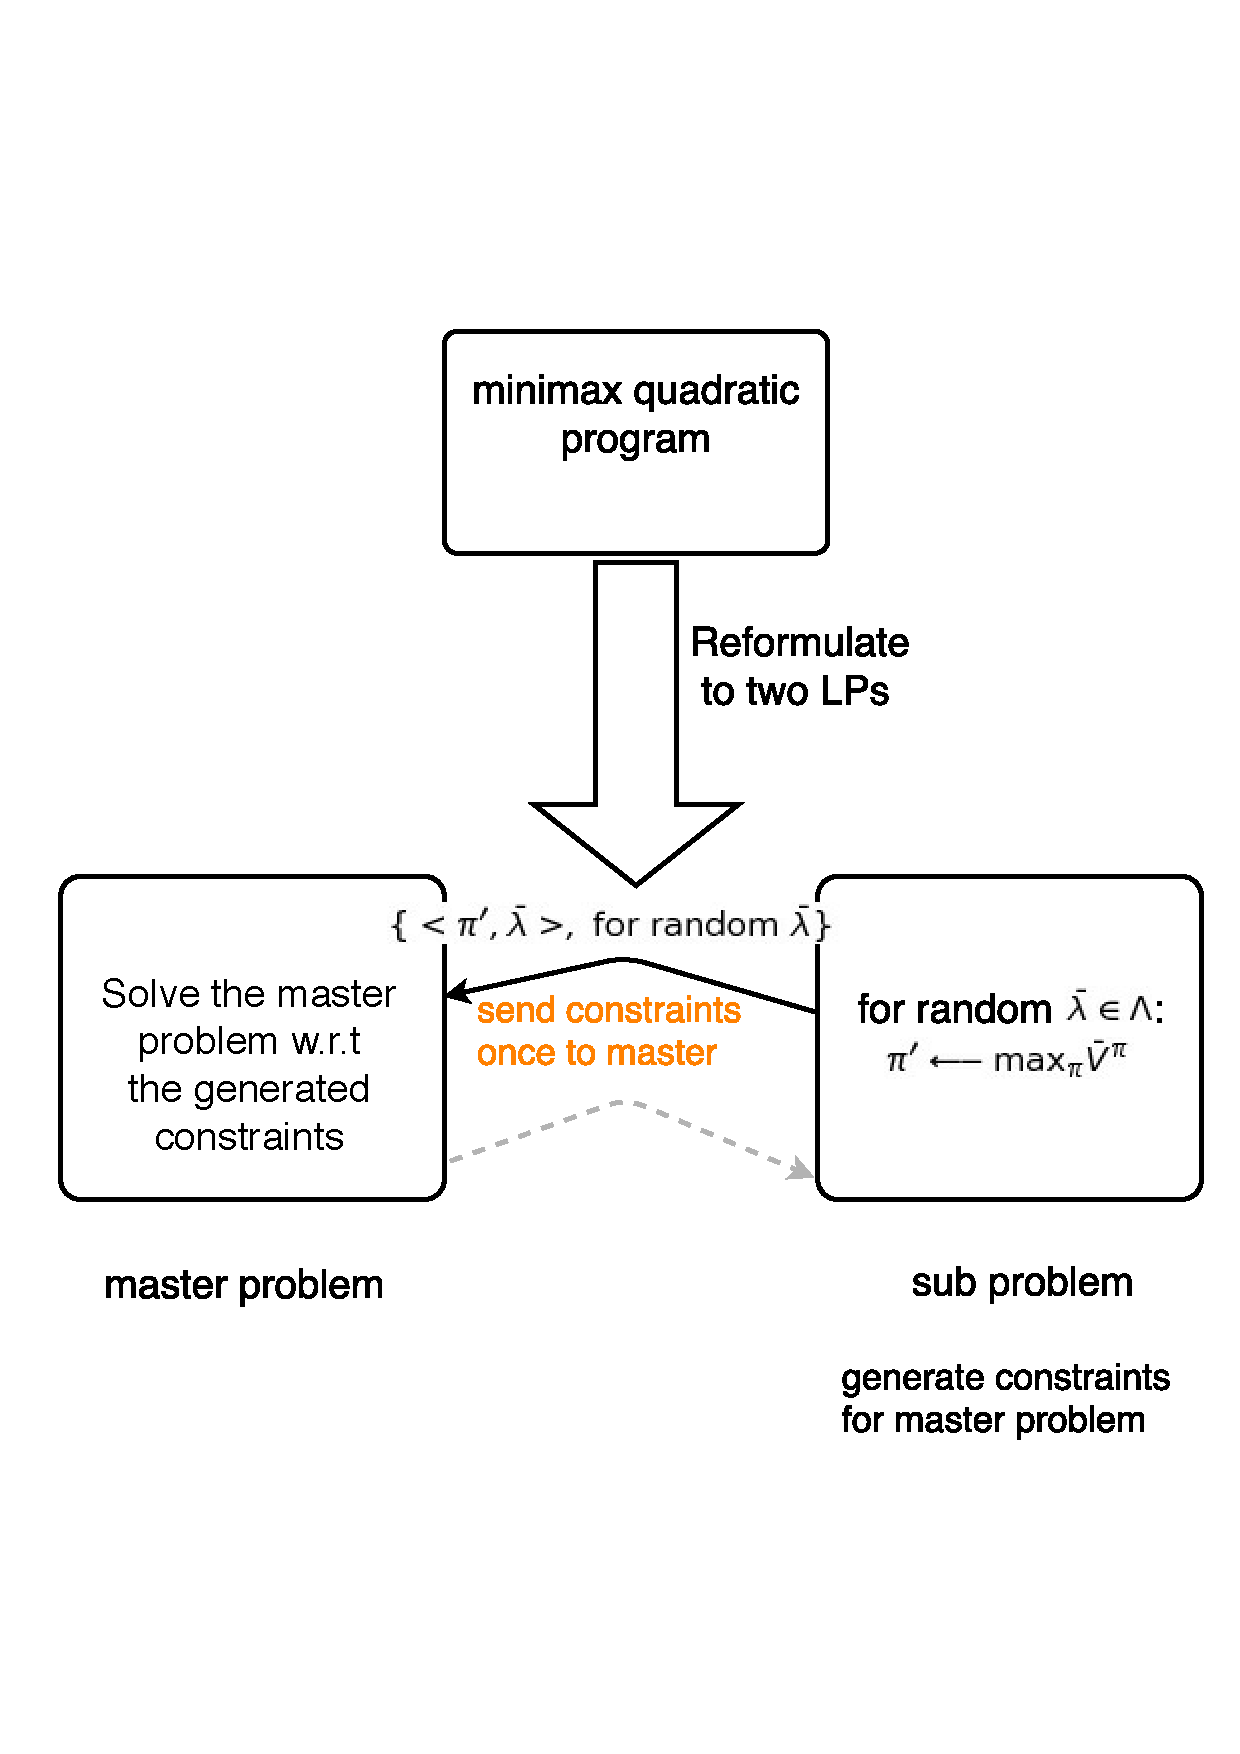
\includegraphics[width=1.1\textwidth]{figures-new/bender}
\end{column}
\end{columns}
\end{frame}

%%%%%%%%%%%%%%%%%%%%%%%%%%%%%%%%%%%%%%%%%%%%%%%%%%%%%%%%%%%%%%%%%%%%%%%%%

\begin{frame}\frametitle{Changing of States and Actions vs calculation time for minimax regret}

%\begin{minipage}{.45\linewidth}
\begin{figure}
\centering
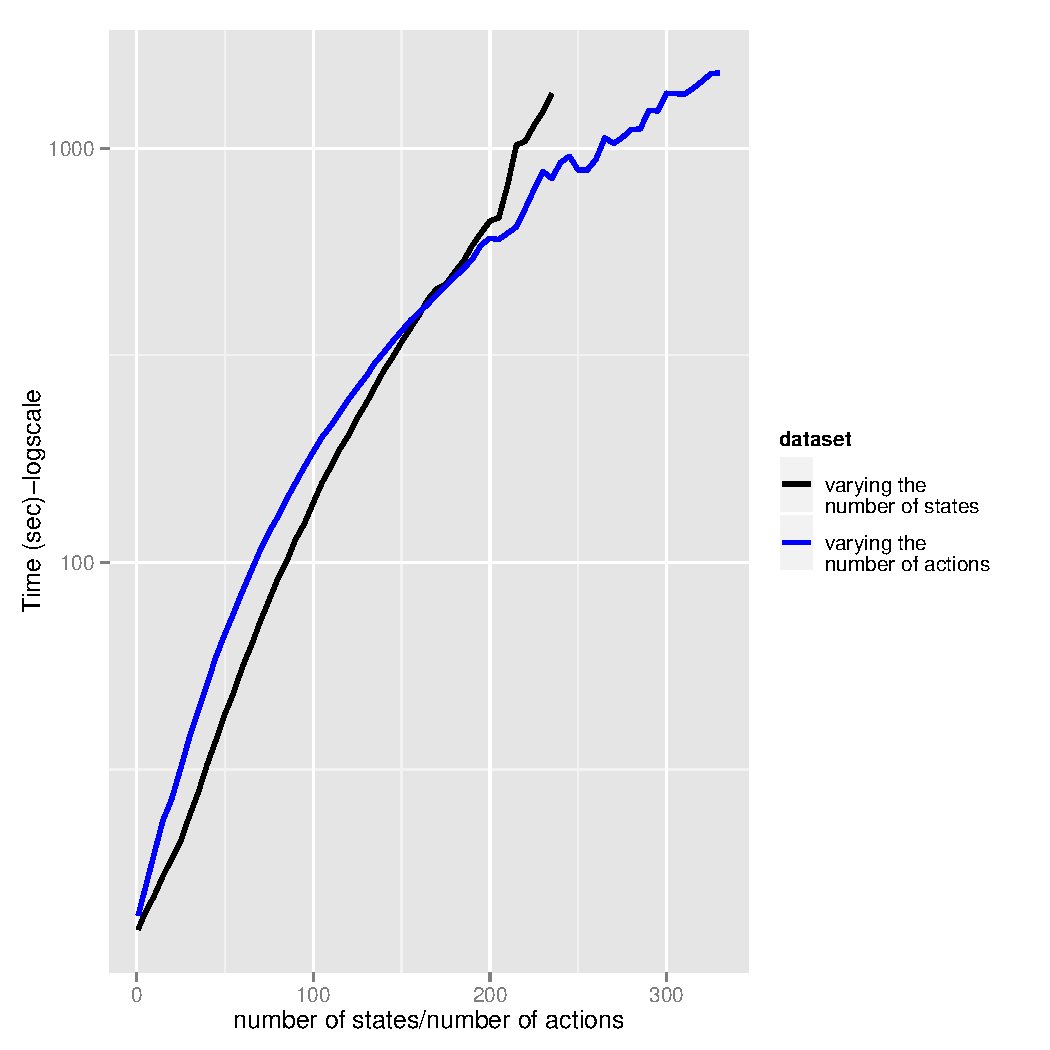
\includegraphics[width=0.6\textwidth]{images/ourresult.pdf}
%\node [align=left] at (-16,6) {$\Lambda$ polytope};
%\node [align=left] at (-14,10) {$\pmb{\lambda}$};
  
\end{figure}
Our method is \textbf{applicable for more than $200$ states}

\end{frame}

%%%%%%%%%%%%%%%%%%%%%%%%%%%%%%%%%
\begin{frame}{Conclusion}

\remark{minimax regret calculation}
\begin{itemize}
\item The selected random points method is \textbf{less complex and computationally faster} than the other methods in the literature.
%\item {\color{red} we wish to:} compute the accuracy of this method.
\end{itemize}
%{\color{red} we wish to:} Implement our methods on social choice and multi agent concepts. 

\end{frame}

%%%%%%%%%%%%%%%%%%%%%%%%%%%%%%%%%%%%

\section{IRMDP Application in Web Service Composition}

%-------------------------------------

\begin{frame}{}
\begin{center}
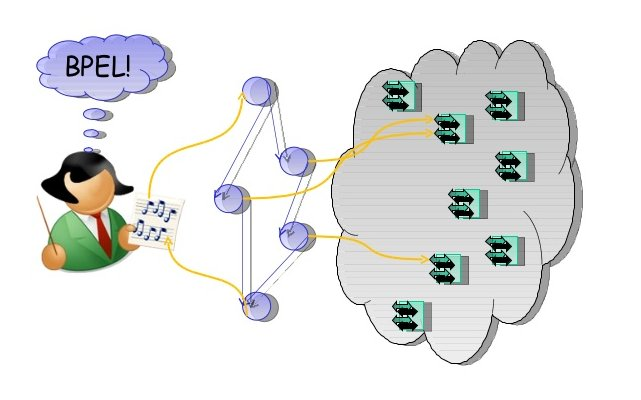
\includegraphics[width=0.6\textwidth]{iimas/ws-composition.jpg}\footnote{the figure comes from Tammo van Lessen et al. presentation}
\end{center}
\end{frame}

%----------------------------------------

\begin{frame}{Goal}
In Internet of Things (IoT) services composition, there are twoe services:
\begin{itemize}
	\item \PA{Abstract Service}: describe the functionality of a service, such as reserving hotel web services or airline web services.
	\item \PA{Concrete Service}: refers to an executed service such a web services as booking.com, easyjet.com and et. 
\end{itemize}

\vspace{0.3cm}

Each concrete service has different Quality of Services (QoS) levels.\\

\vspace{0.3cm}

\remark{Question}: 

\begin{itemize}
	\item for each abstract service, what concrete services should be selected 
	\item what is the best abstract services permutation in the user’s task in
order to satisfy the user's requirements in terms of the QoS ?
	\item Qos has various attributes example: response time, throughput 
\end{itemize}

\end{frame}

%-------------------------------------
\begin{frame}[plain]
\vspace{0.3cm}
The advantage based value Iteration algorithm is implemented on real data base of Web services executions \cite{•}\\
	\begin{center}
	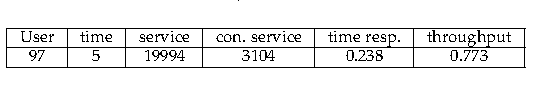
\includegraphics[width=0.6\textwidth]{iimas/table-line.pdf}\\
	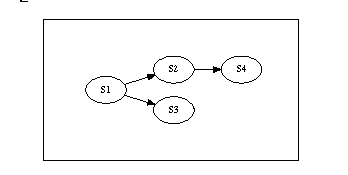
\includegraphics[width=0.5\textwidth]{iimas/states.pdf}\\
	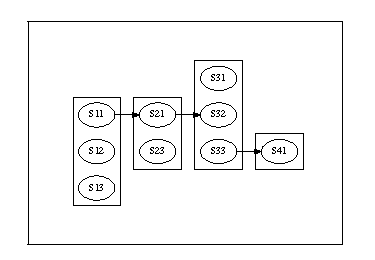
\includegraphics[width=0.5\textwidth]{iimas/actions-ws.pdf}\\
	\end{center}
		
\end{frame}

%-------------------------------------

\begin{frame}\frametitle{How model Web Service Composition as MDP}
A \textbf{VMDP-Service Composition (VMDP-SC} is a tuple $(T, AS, CS, P_t(.|as,cs), \bar{r}_t, AS_T)$, where  

\begin{itemize}
\item[ -] \textbf{MDP horizon length} $T= 1 \cdots N$ is a total number of time stages. 
\item[-] \textbf{states:} $AS$ is set of \remark{abstract services}.
\item[-] \textbf{actions}: $CS$ is set of \remark{ concrete services}.
\item[-] \textbf{probability function:} $P_t(S_j | S_i, S_{ik} )$ is the probability of invoking the concrete service $S_{ik}$ for abstract activity $S_i$ and resulting in the abstract activity $S_j$.
\item[-] \textbf{reward function:} $ \overline{r}_t: AS \times CS \longrightarrow \mathbb{R}^d$: reward function. %The $\overline{Q}(S_i, S_{ik})$ reward is the generated Q vector value after invoking $S_{ik}$ in $S_i$ at time step $t$. Given that 
$d$ is the number of QoS criteria, we obtain $\overline{r}_t(S_i, S_{ik}) = ({r_1}_t(S_i, S_{ik}), \cdots, {r_d}_t(S_i, S_{ik}))$. 
\item[-] \textbf{terminal states}: $AS_T$ is the set of terminal services. 

\end{itemize}

\end{frame}
%------------------------------------
\begin{frame}{Experimental Results}
All experiments are on sequential form of abstract service connection. 
	\begin{center}
	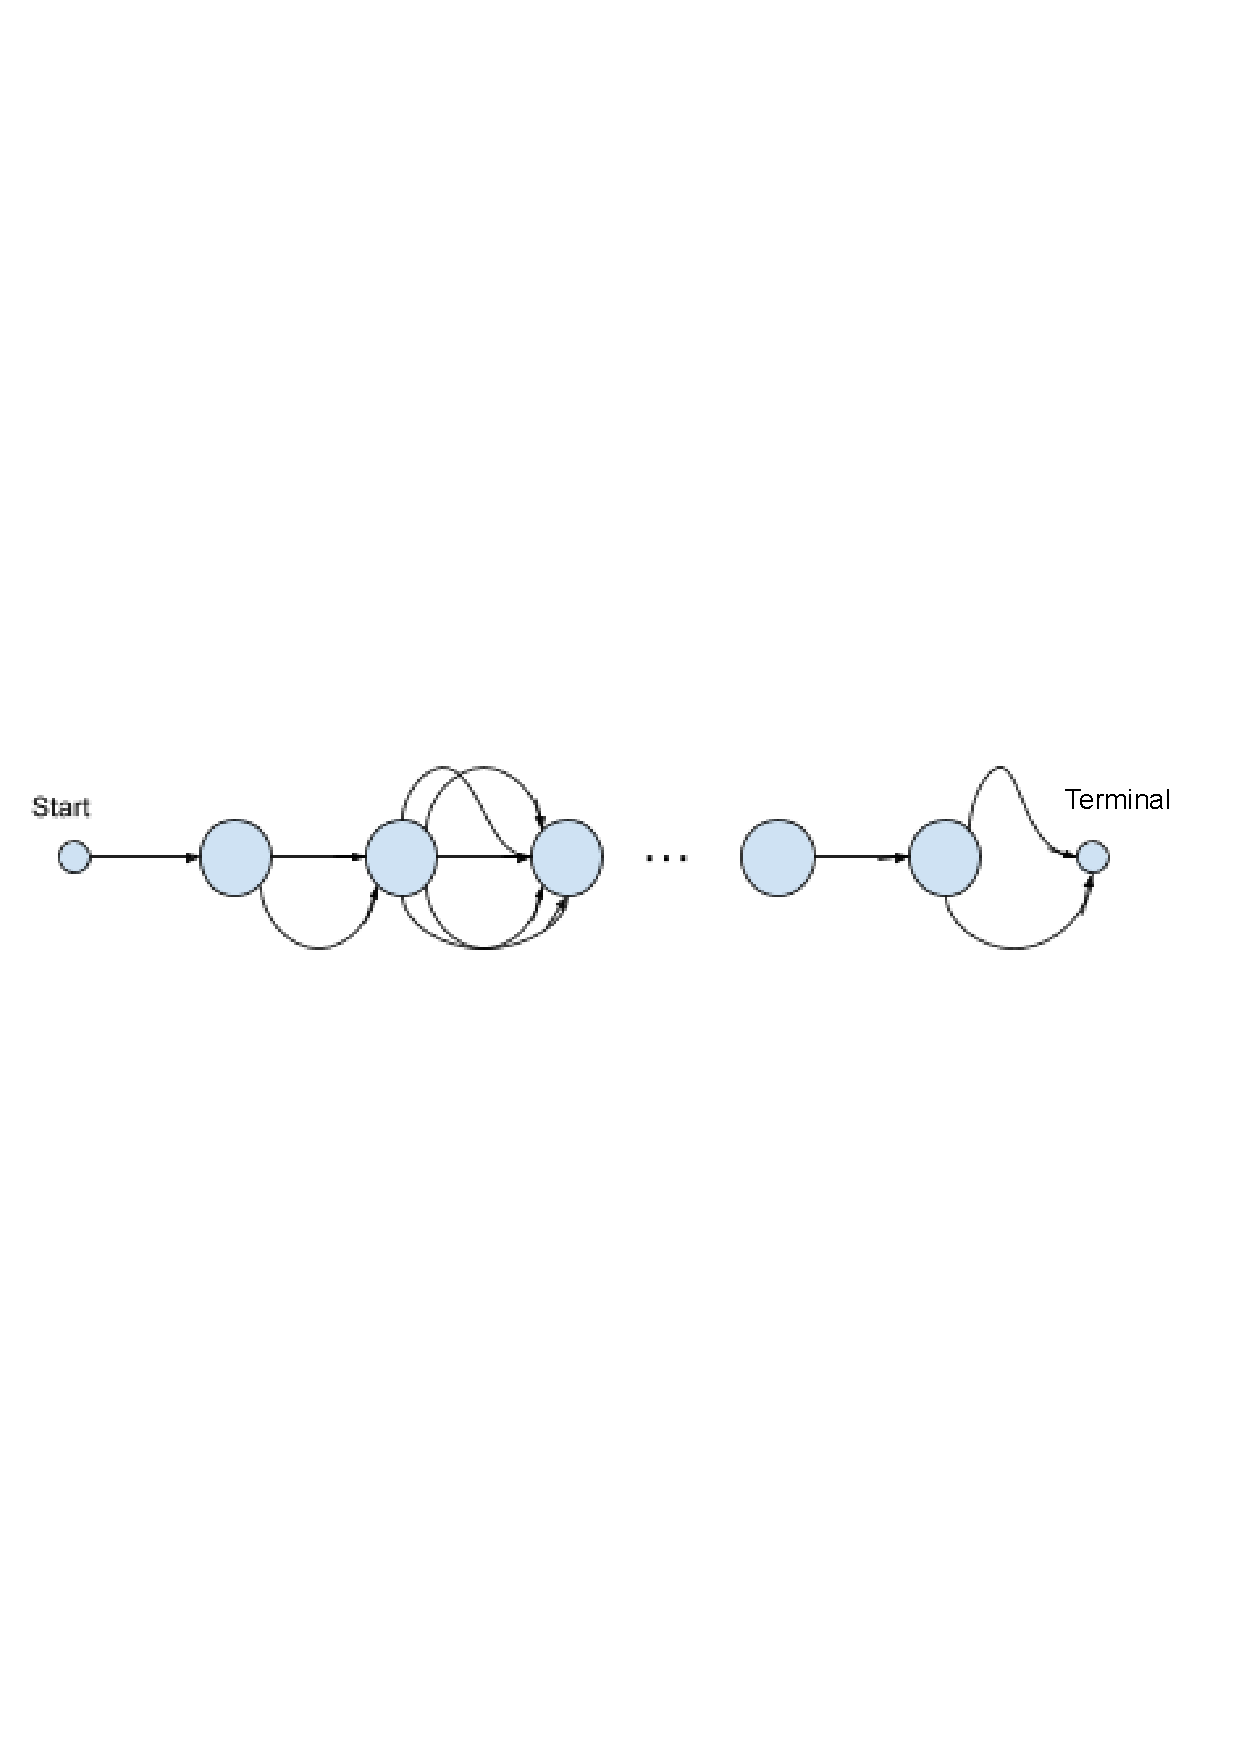
\includegraphics[width=0.8\textwidth]{iimas/seq-mdp-.pdf}
	\end{center}
	we have a VMDP-SC with the following parameters:
\begin{itemize}
\item[-] number of \textbf{episodes}:  $N=64$
\item[-] $744$ number of abstract services 
\item[-] $3551$ total number of concrete services (in our case web services)
\item[-] The transition function and terminal states depend on the proposed model or relation types among the abstract services. 
\item[-] $\overline{r}_t \in \mathbb{R}^2$ with two quality of services: response time and throughout 
\end{itemize}
\end{frame}

%------------------------------------
\begin{frame}{Experimental Results}
\begin{table}
\begin{tabular}{ l | l | }
  user & weight vector \\
  \toprule
   $\bar{W}_0$ & $[0.319797998295 \;\;\;\;\;\;\;\;, \;\;\;\;\;\;\;\; 0.680202001705]$ \\
   $\bar{W}_1$ & $[0.8573741847324399 , 0.14262581526756013]$ \\
   $\bar{W}_2$ & $[0.1696287781131175\;,\; 0.8303712218868825]$ \\
   $\bar{W}_3$ & $[0.6451844883834318\;,\; 0.3548155116165682]$\\
   $\bar{W}_4$ & $[0.47245438345\;\;\;\;\;\;\;\;\;\; , \;\;\;\;\;\;\;\;\;\; 0.52754561655]$\\ 
 \end{tabular} 
 \caption{The weight vectors for $5$ system users with various preferences on the attributes (throughput, response time).} 
 \label{table:weights}
\end{table}
\end{frame}


%------------------------------------
\begin{frame}
	\begin{figure}[t]
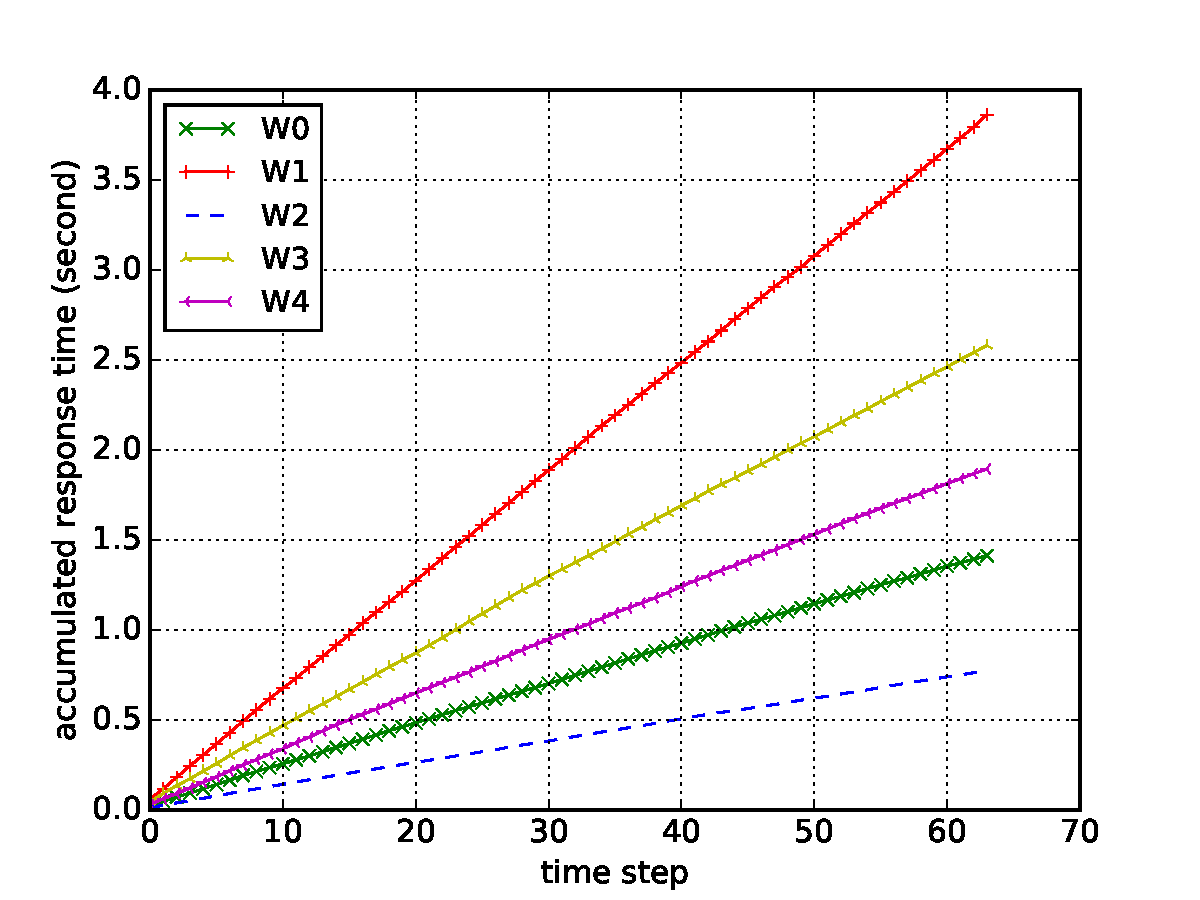
\includegraphics[width=8cm]{iimas/rt_step_all++.pdf}
\caption{This figures demonstrate how the accumulated response time increases during each time step. The weight preferences are based on table~\ref{table:weights}.} 
\centering
\label{fig:rt-vs-timestep}
\end{figure}
%%%%%%% 
\end{frame}

%----------------------------------
\begin{frame}

\begin{figure}[t]
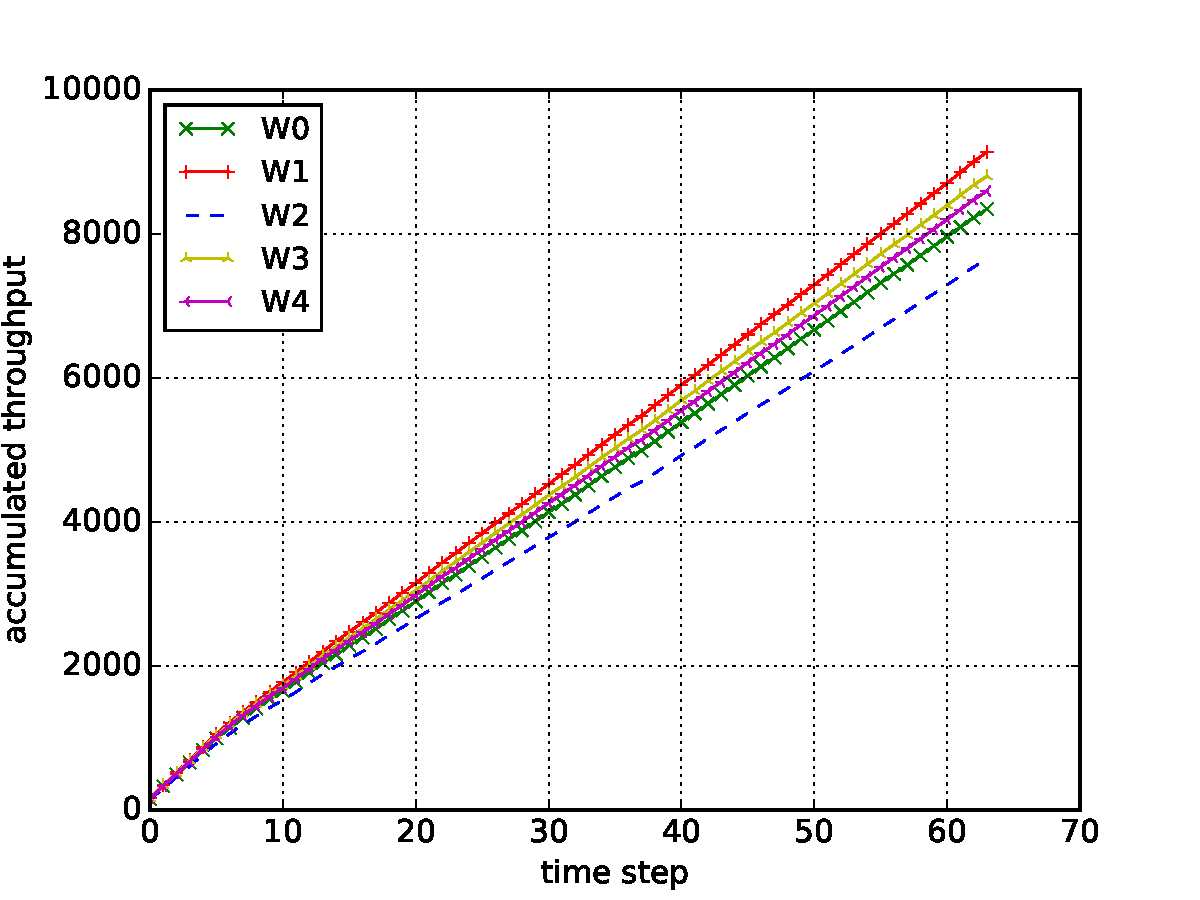
\includegraphics[width=8cm]{iimas/trough_step_all++.pdf}
\caption{this demonstrates how the accumulated throughout increases during each time step. The weight preferences are based on table~\ref{table:weights}.}
\centering
\label{fig:trput-vs-timestep}
\end{figure}
\end{frame}
%-----------------------------------
\begin{frame}
\begin{figure}[t]
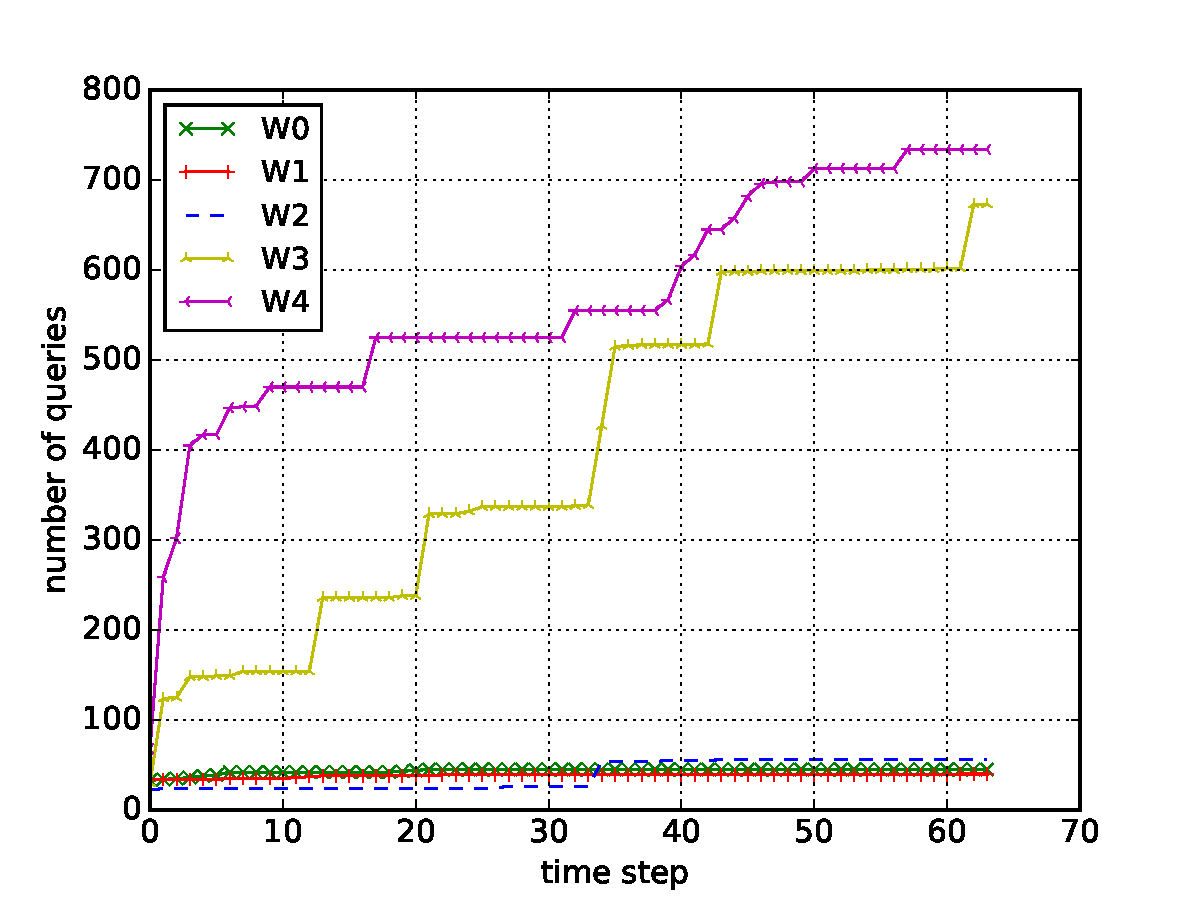
\includegraphics[width=8cm]{iimas/time-queries-all++.pdf}
\caption{This figure shows the number of queries proposed to the user during each time step. The weight preferences are based on table~\ref{table:weights}.}
\centering
\label{fig:queries-vs-timestep}
\end{figure}
\end{frame}
%------------------------------------
\begin{frame}{Conclusion}

\end{frame}

%------------------------------------
\begin{frame}
	\begin{center}
	Information Extraction from Internet Using Deep Reinforcement Learning Approach
	\end{center}
\end{frame}

%-------------------------------------
\section{Information Extraction from Internet Using Deep Reinforcement Learning Approach}
\begin{frame}{Project Goal}
\begin{center}
Receive a person's name from DataBase supported by Sociologists \\
	$\Downarrow$\\
	%\vspace{0.3cm}
		\fbox{Our System}\\
	%\vspace{0.3cm}	
	$\Downarrow$\\
	The person's professional history
\end{center}
\PA{Example}: John Smith : 2012 Edinburgh University - 2014 Sussex University - 2016 IBM - 2017 Bosch

\PA{How to test the system}: John Smith + his destination is given in the DB \\
John Smith left Mexico to \remark{Edinburgh University 2012} to do a PHD
in \remark{Computer Vision}\\
\vspace{0.5cm}
If \textbf{Edinburgh University} and \textbf{2012} are in our result $\longrightarrow$ The system
works correctly

\end{frame}

%------------------------------------------------
\begin{frame}
\begin{center}
	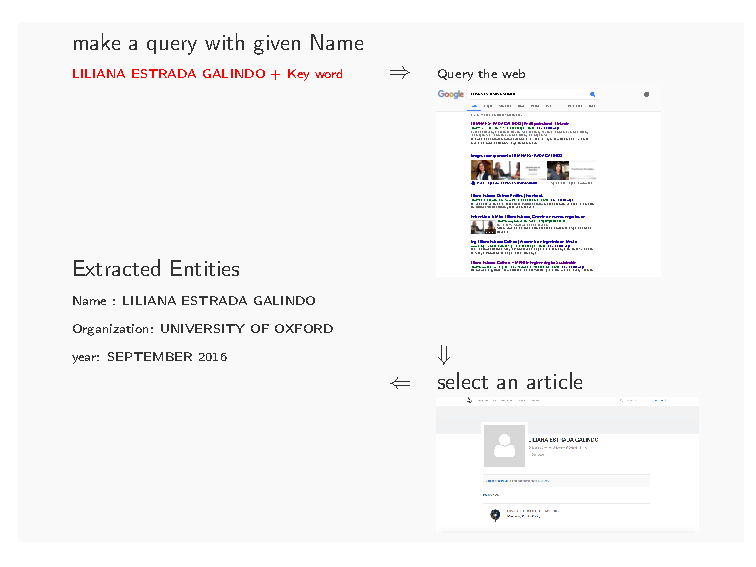
\includegraphics[width=12cm]{iimas/query.pdf}
\end{center}
\end{frame}

%-----------------------------------------------
\begin{frame}{Question}
	\begin{center}
		When should we ask queries and when should we improve the
		entities based on the already existed articles?
	\end{center}
\end{frame}

%------------------------------------------------
\begin{frame}{Queries and Extracted Entities}
Query types for a given name:
\begin{itemize}
	\item name, 
	\item name | PHD
	\item name | doctorate,
	\item name | master,
	\item name | undergraduate,
	\item name | university,
	\item name | institute
\end{itemize}
\vspace{0.3cm}
Search engines: Google, Bing, DuckDuckGo and Citeseer\\
Send name $\longrightarrow$ \PA{generate query} + person's name $\longrightarrow$ get first 20 articles \\
\vspace{0.3cm}
Extract three entities from each article:\\
\remark{Person's name, Organisation name, year- time}

\end{frame}
%------------------------------------------------
\begin{frame}{Challenges}
\begin{center}
	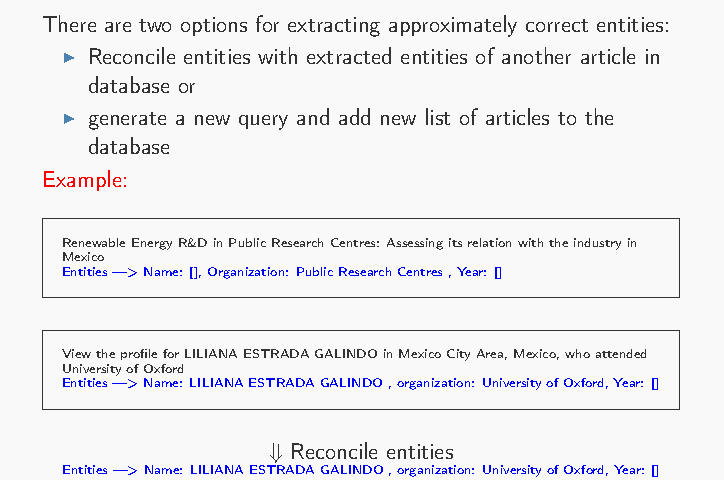
\includegraphics[width=11cm]{iimas/options.pdf}
\end{center}
\end{frame}

%------------------------------------------------
\begin{frame}{Markov Decision Process}
\begin{center}
	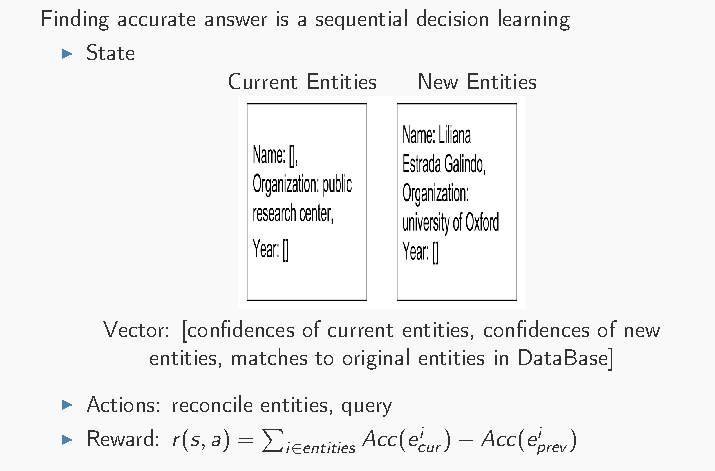
\includegraphics[width=11cm]{iimas/mdp.pdf}
\end{center}
\end{frame}

%------------------------------------------------
\begin{frame}{Actions in MDP}
\begin{center}
	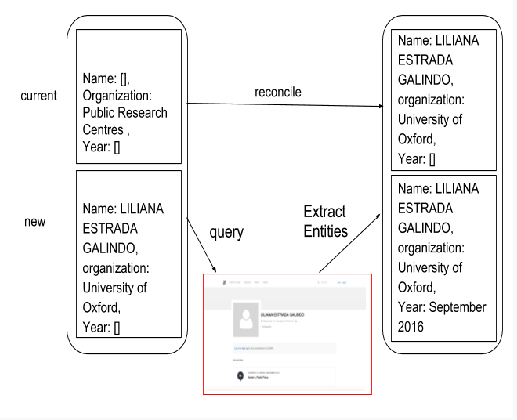
\includegraphics[width=10cm]{iimas/actions.pdf}
\end{center}
\end{frame}

%------------------------------------------------

\begin{frame}{Question}

\begin{center}
How get the most accurate extracted entities by generating as few
number of queries?
\end{center}

\end{frame}

%------------------------------------------------
\begin{frame}{Q-learning}
Best solution maximizes expected reward in each episode $Q: S \times A \longrightarrow \mathbb{R}$ evaluates the value of selecting action $a$ in state $s$. \\
\vspace{0.3cm}
An iterative method that finds the best action in each state: 
\begin{align*}
Q(s_t, a_t) = Q(s_t, a_t) + \alpha [r_t + \gamma \text{max}_a Q(s_{t+1}, a) - Q(s_t, a_t)]
\end{align*}
Optimal Policy: 

\begin{align*}
a = \text{argmax}_a Q(s,a)
\end{align*}

\end{frame}

%------------------------------------------------
\begin{frame}{Q Learning}
\begin{center}
	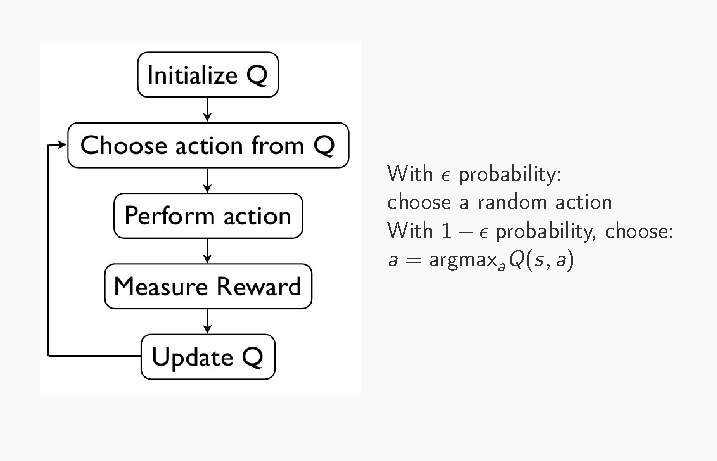
\includegraphics[width=11cm]{iimas/q-learning.pdf}
\end{center}
\end{frame}

%------------------------------------------------
\begin{frame}{Deep Q Networkx}
\begin{center}
	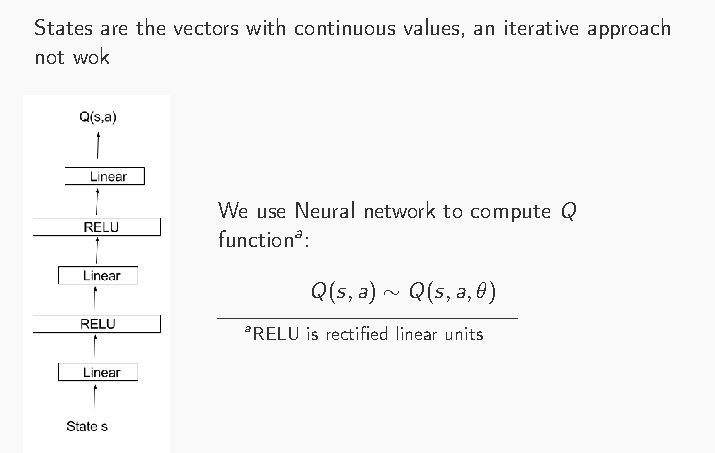
\includegraphics[width=11cm]{iimas/dqn.pdf}
\end{center}
\end{frame}

%------------------------------------------------

\begin{frame}{Ongoing Works}

\end{frame}

%------------------------------------------------

\begin{frame}{Conclusion}

\end{frame}

%------------------------------------------------

\section{An Automatic System for Extracting Information from Multi-party dialogues}
\begin{frame}{REUS Project \hspace*{7.1cm}~ 
\includegraphics[width=0.8cm]{images/reus.png}}

\begin{figure}
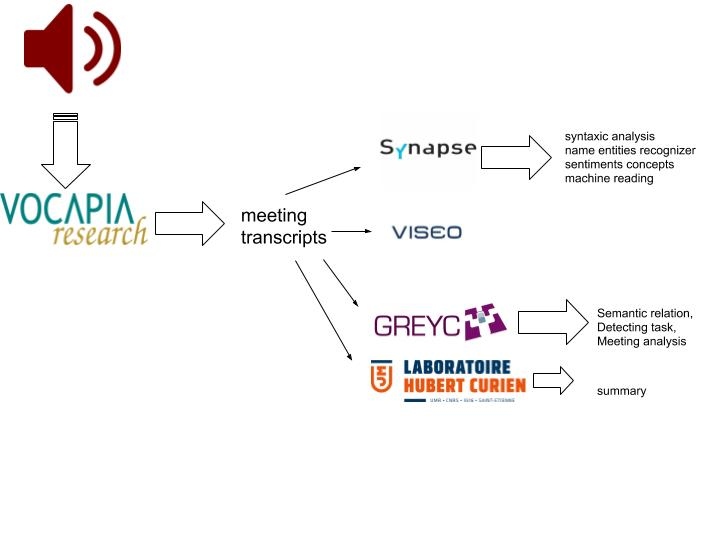
\includegraphics[width=12cm]{images/reus-.jpg}
\end{figure}

\end{frame}
%%%%%%

\begin{frame}\frametitle{Challenges and Difficulties} 
\begin{figure}
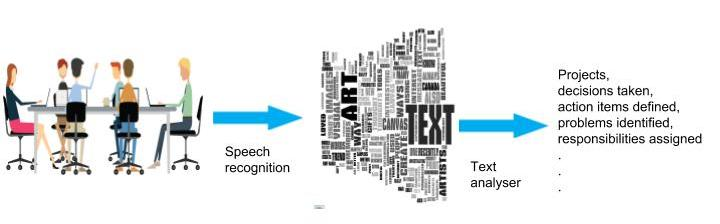
\includegraphics[width=12cm]{images/reus-image.jpg}
\end{figure}

output of speech recognition methods includes:
\begin{itemize}
\item  unstructured word streams
\item weak punctuation
\item weak formatting
\item or capitalizations
\end{itemize}


\end{frame}
%%%

%------------------------------------------------
\begin{frame}

Two main works on this project:
\begin{itemize}
	\item \remark{Topic and Information Extraction}: Extracting important information and topics from meeting based corpus
	\item \remark{Dialogue Act Tagging}: Tagging dialogue acts of meetings using unsupervised learning approaches. 
\end{itemize}

\end{frame}

%%%%%%%%%%%%%

\begin{frame}
\begin{center}
\textbf{Topic and Information Extraction}
\end{center}
\end{frame}

%%%%%%%%%%%%%

\begin{frame}\frametitle{extracting information and topics}

\imp{GOAL:} find answers for the following questions:
\begin{itemize}
\item Can we \textbf{identify the specific terms} for an \textbf{individual meeting} in comparison to \textbf{thematically related} but distinct meetings?
\item \textbf{How group meetings together} by identifying \textbf{participants' names} or their \textbf{manner of speech}?
\item \textbf{How close} are the extracted words to the \textbf{provided goal standards (summaries)}?
\end{itemize}

\end{frame} 
%%%%%

\begin{frame}
We used two approaches for extracting information from \remark{Augmented multi-party interaction \textbf{(AMI)} Corpus Structure}: 

\begin{columns}[T] % contents are top vertically aligned
\begin{column}[T]{8cm} % each column can also be its own environment

\begin{itemize}
	\item \textbf{Counting Stochastic}: Term Frequency - Inverse Document Frequency
(tf-idf): $\text{tf-idf}(w, d,D) = \text{tf}(w, d)\text{idf}(w,d)
$ \\where $\text{idf}(w,D) = \log \frac{N}{1+|d\in D \; s.t. \; w \in d|}$ for $N$ number of documents
\end{itemize}
     
     \end{column}
\begin{column}[T]{3cm} % alternative top-align that's better for graphics
          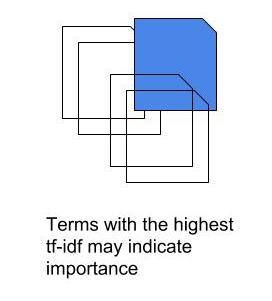
\includegraphics[height=3cm]{images/tf-idf.jpg}
\end{column}
\end{columns}

\begin{itemize}
		\item \textbf{Topic Modeling}: Non-negative Matrix Factorization (NMF): \\
		$\mathbf{V} \in \mathbb{R}^{m \times n}$ \imp{$m$}: unique words in a corpus of \imp{$n$} meetings (documents). \remark{Goal} $\mathbf{V} \sim \mathbf{WH}$ where 
$\mathbf{W} \in \mathbb{R}^{m \times k}$ and $\mathbf{H} \in \mathbb{R}^{k \times n}$

\end{itemize}
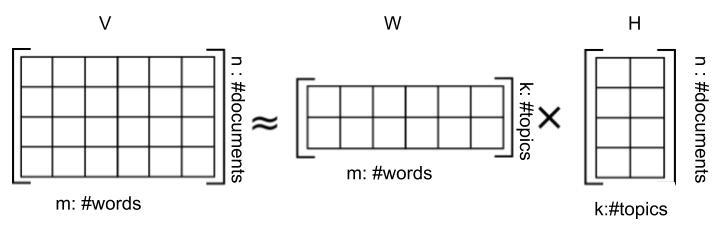
\includegraphics[height=3.5cm]{images/nmf-.jpg}
\end{frame}

%------------------------------------------------
\begin{frame}{tf-idf}
We extract different types of information, respecting different regroupment on meetings

\begin{columns}[T] % contents are top vertically aligned
\begin{column}[T]{7cm} % each column can also be its own environment

\begin{itemize}
\item Characterising individual meetings Extracted words indicates that:
 \begin{itemize}
 	\item groups are close in the beginning and in the end
 	\item groups diverge in the middle. 
 \end{itemize}
\item Grouping meetings:
	\begin{itemize}
		\item same groups of meetings have same name combinations.
		\item same groups of meetings have same participants’ \textbf{manner of speech} such as extracted words: \textbf{you’ll}, \textbf{ain’t} and \textbf{shoulda}
\end{itemize}	 
\end{itemize}

\end{column}
%
\begin{column}[T]{4cm}
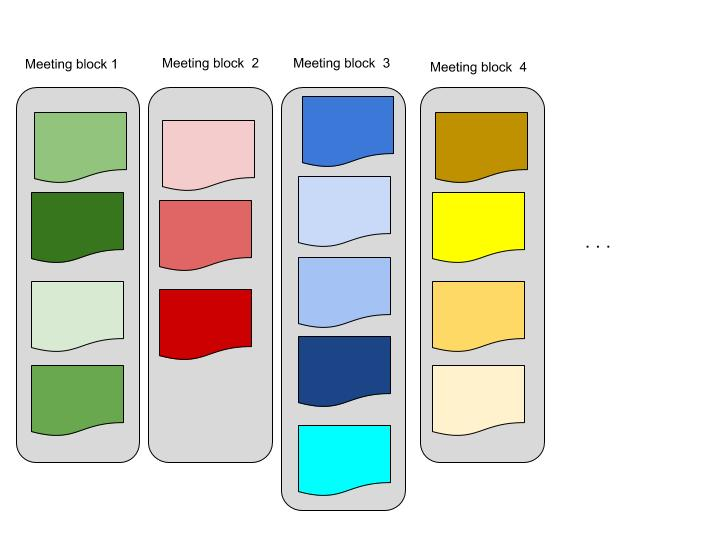
\includegraphics[height=3cm]{images/charac-tf-idf-.jpg}\\
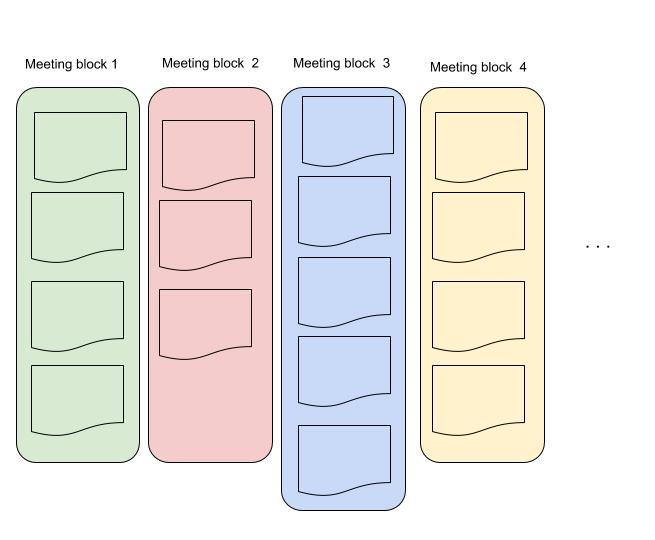
\includegraphics[height=3.5cm]{images/group-tf-idf.jpg}

\end{column}
\end{columns}

\end{frame}

%%%%%%%%%%%%%%%%%%%%%%%%
\begin{frame}[plain]
\frametitle{abstractive and extractive accuracies: \tfidf{} vs. \NMF{}}
%extractive accuracy is higher than abstractive accuracy\\
extractive-abstractive accuracy ratio for \NMF{} ($\mathbf{2.1}$) is \textbf{lower} than extractive-abstractive accuracy ratio for \tfidf{} ($\mathbf{4.65}$)
\begin{figure}[!htb]
\centering
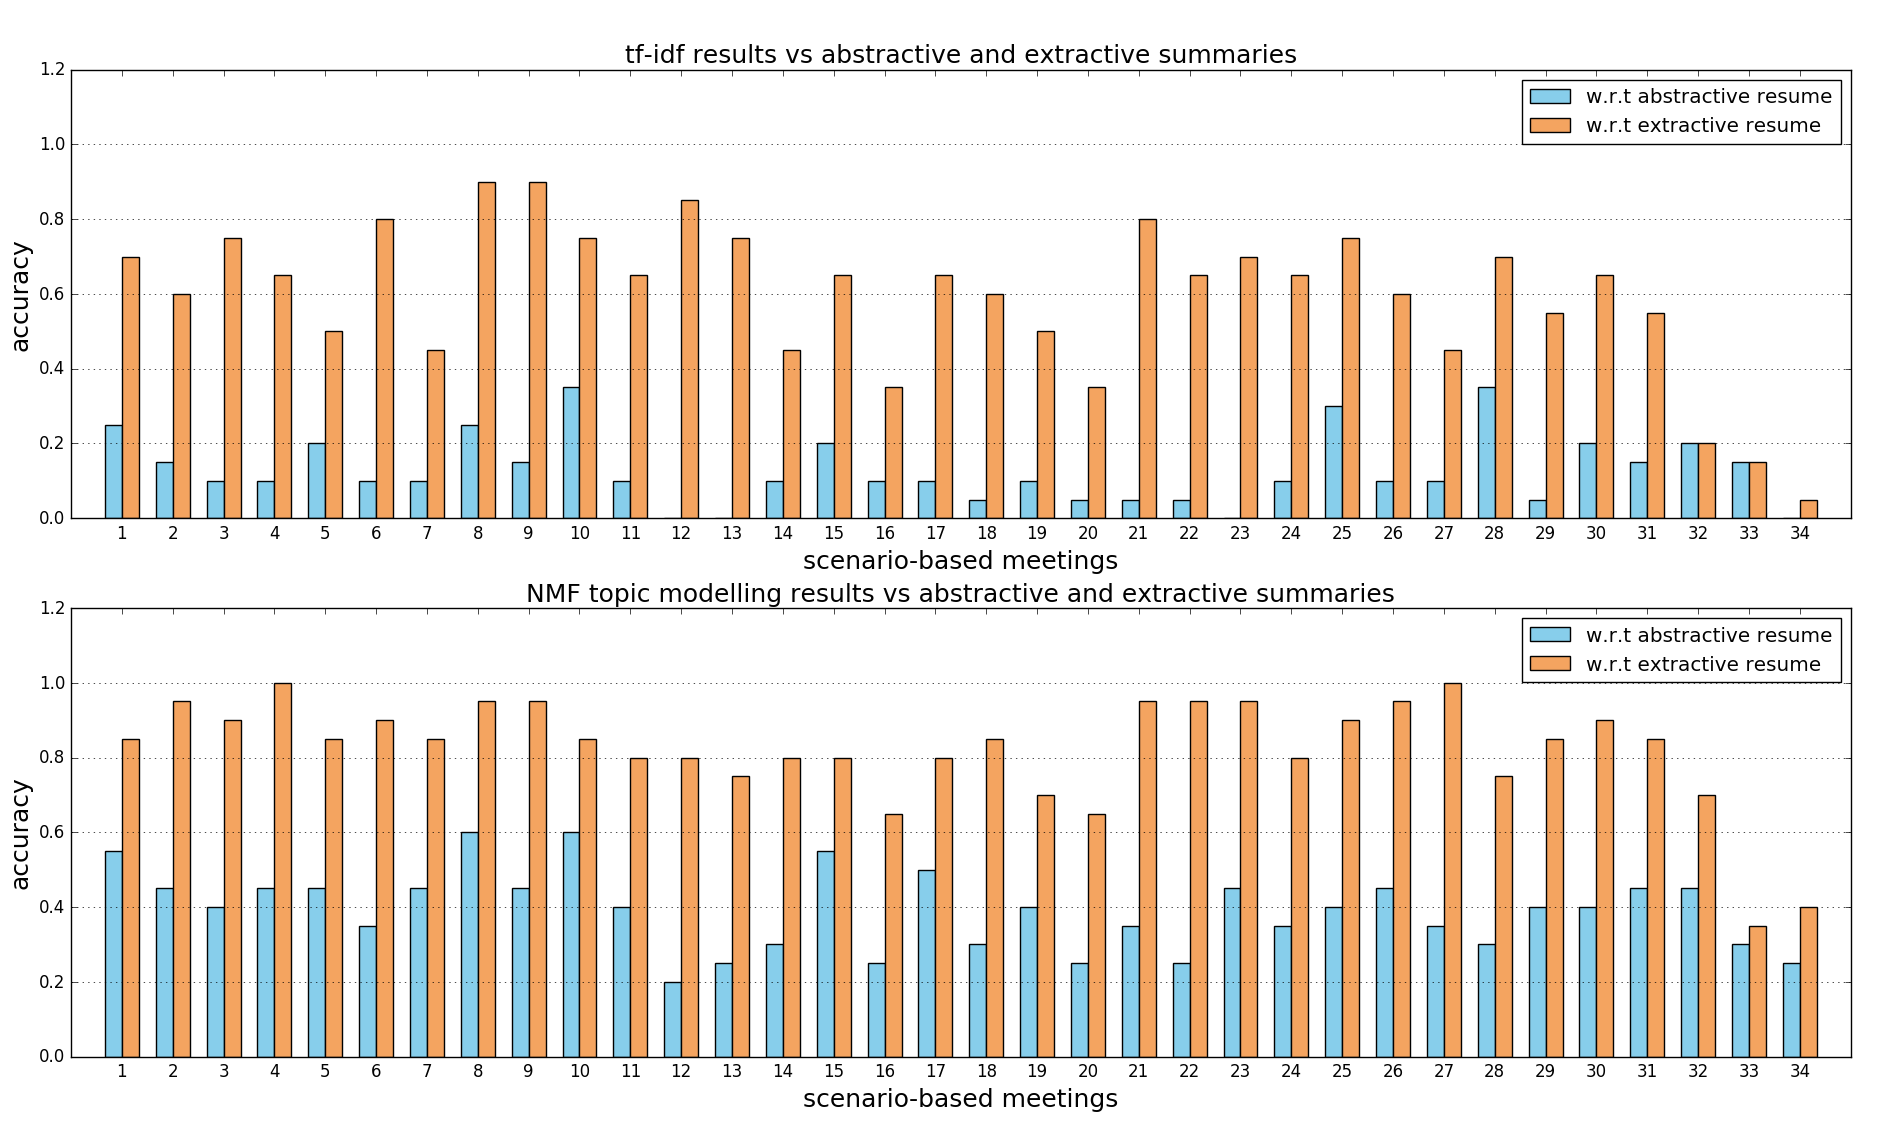
\includegraphics[width=12cm]{images/tfidf-nmf.png} %l'image est réduite de moitié
\label{fig:tf-idf-scenario}
\end{figure}

\end{frame}


%%%%
\begin{frame}%[plain]
\frametitle{Conclusions}
\begin{itemize}

\item \textbf{topic modeling is better} for \textbf{summarization and theme extraction} within a set of \textbf{thematically related meetings} acted out by \textbf{different groups of participants}.

\item \textbf{\tfidf{} performs well} on \textbf{meeting characterisations} and \textbf{speaker identification} within a \textbf{meeting acted out by a single group} speaking about the same scenario.

\item the information derived the \textbf{tf-idf score} and the \textbf{topic modeling} \textbf{are complementary}.
\end{itemize}

\end{frame}

%%%%%%%%%%%%%

\begin{frame}
\begin{center}
\textbf{Dialogue Act Tagging using Unsupervised Learning Approaches}
\end{center}
\end{frame}

%%%%%%%%%%%%%
\begin{frame}{Fragment of labelled conversation (from multi-party dialogue corpus (Switchboard Corpus))}


\begin{center}
\scalebox{0.8}{
\begin{tabular}{ lc lc lc }
 Speaker & Dialogue Act & Utterance \\ \hline
 A & YES-NO QUESTION & \small{So, do you go to college right now?} \\  
 A & ABANDONED & Are you-, \\  
 B & YES-ANSWER  & Yeah, \\  
 B & STATEMENT &  It's my last year [laughter].\\    
 A & DECLARATIVE QUESTION & you're a, so you're a senior now. \\  
 B & YES-ANSWER & yeah, \\  
 B & STATEMENT &  \makecell{I'm working on my projects, trying \\ to graduate [laughter].}\\  

 A & APPRECIATION & oh, good for you. \\  
 B & BACKCHANNEL &  yeah \\  
 A & APPRECIATION &  That's good.\\  
 A & YES-NO-QUESTION & um, is, is NC university is that, State,\\  
 B & STATEMENT &   NC state. \\  
 A & SIGNAL-NON-UNDERSTANDING & What did you say? \\
 B & STATEMENT	& NC state. \\   
\end{tabular}
}
\end{center}

\end{frame}
%%%%%%%%%%%%
\begin{frame}
To define dialogue act tagging using unsupervised approaches:
\begin{itemize}
 \item \textbf{which set of dialogue acts}
 \item how \textbf{represent texts as numerical vectors} in order to implement unsupervised machine learning methods?
\item \textbf{which unsupervised methods }should we use?
\item \textbf{How to label }extracted \textbf{clusters }or groups from unsupervised learning approaches?
\item \textbf{How }should we \textbf{evaluate our results} 
\end{itemize}

\end{frame}

%------------------------------------------------
\section{Minmax Regret based Approach for Computing Optimal Deterministic Policies}

%------------------------------------------------

\begin{frame}{}

\end{frame}

%------------------------------------------------

\begin{frame}
\frametitle{References}
\footnotesize{
\begin{thebibliography}{99} % Beamer does not support BibTeX so references must be inserted manually as below
\bibitem[Hsueh, 2008]{hsueh2008} P. Y. Hsueh and J. Moore. (2008)
\newblock Automatic decision detection in meeting speech.
\newblock \emph{Machine Learning for Multimodal Interaction.}
%%%
\bibitem[bui, 2009]{bui2009}T. H. Bui, M. Frampton, J. Dowding, and S. Peters.   (2009)
\newblock from multi-party dialogue using directed graphical models and semantic similarity.
\newblock \emph{}
%%%
\bibitem[Fernandez, 2008]{Fernandez2008} R. Fernandez, M. Frampton, P. Ehlen, M. Purver, and S. Peters. (2008)
\newblock Modeling and detecting decisions in multi-party dialogue.
\newblock \emph{}
%%%

\bibitem[Dowding, 1993]{Dowding1993}J. Dowding, J. M. Gawron, D. Appelt, J. Bear, L. Cherny,
R. Moore, and D. Moran. (1993)
\newblock GEMINI: a natural language system for spoken-language understanding
\newblock \emph{ACL}
%%%%
\bibitem[Godfrey, 1992]{Godfrey1992}John J Godfrey, Edward C Holliman, and Jane McDaniel.
\newblock Switchboard: Telephone speech corpus for research and development.
\newblock \emph{ICASSP-92}
%%%%%
\bibitem[Collobert, 2011]{Collobert2011}Ronan Collobert, Jason Weston, Leon Bottou, Michael Karlen, Koray Kavukcuoglu, and Pavel Kuksa. (2011)
\newblock Natural language processing (almost) from scratch. 
\newblock \emph{The Journal of Machine Learning Research}
%%%%%
\bibitem[Kalchbrenner 2013]{Kalchbrenner2013}Nal Kalchbrenner and Phil Blunsom. (2013)
\newblock Recurrent convolutional neural networks for discourse compositionality
\newblock \emph{}

%\bibitem[]{}
%\newblock
%\newblock \emph{}
\end{thebibliography}
}
\end{frame}

%------------------------------------------------
\begin{frame}
\frametitle{References}
\footnotesize{
\begin{thebibliography}{99} 

\bibitem[Ji, 2016]{Ji2016}Ji Young Lee and Franck Dernoncourt. (2016)
\newblock Sequential short-text classification with recurrent and convolutional neural networks.
\newblock \emph{}
%%%
\bibitem[Kim et al.2015]{Kim2015} Seokhwan Kim, Luis Fernando D'Haro,
Rafael E. Banchs, Jason Williams, and Matthew Henderson. (2015)
\newblock Dialog  State  Tracking  Challenge  4: Handbook.
\newblock \emph{}
%%%
\bibitem[Kim et al.2016]{Kim2016} Seokhwan Kim, Luis Fernando D'Haro,
Rafael E. Banchs, Jason Williams, and Matthew Henderson. (2016)
\newblock The Fourth Dialog State Tracking Challenge
\newblock \emph{In Proceedings of the 7th International Workshop on Spoken Dialogue Systems (IWSDS)}
%%%

%\bibitem[]{}
%\newblock
%\newblock \emph{}
\end{thebibliography}
}
\end{frame}

%----------------------------------------------------------------------------------------

\end{document} 
